% IEEE IoT Journal layout (two-column) — compile from Section-tex/:
%   pdflatex main-ieee.tex && bibtex main-ieee && pdflatex main-ieee.tex && pdflatex main-ieee.tex
% IEEE Internet of Things Journal (two-column) — AN-107
\documentclass[journal]{IEEEtran}
\makeatletter
\newcommand{\journal}[1]{\def\@journal{#1}}
\makeatother
\journal{IEEE Internet of Things Journal}
\providecommand{\IEEEcopyrightnotice}{%
  \copyright{} 2026 IEEE. Personal use is permitted, but republication/redistribution requires IEEE permission.%
}

% Shared packages (article + IEEE builds).
\usepackage{fix-cm}
\usepackage[T1]{fontenc}
\usepackage{lmodern}
\usepackage[utf8]{inputenc}
\usepackage[english]{babel}
\IfFileExists{microtype.sty}{%
  \usepackage{microtype}%
  \microtypesetup{nopatch={verbatim}}%
}{}
\usepackage{listings}
\lstdefinestyle{csnippet}{%
  basicstyle=\scriptsize\ttfamily,%
  breaklines=true,%
  breakatwhitespace=true,%
  columns=fullflexible,%
  keepspaces=true,%
  showstringspaces=false,%
  frame=single,%
  framerule=0.4pt,%
  xleftmargin=0.5em,%
  xrightmargin=0.5em,%
  linewidth=0.96\linewidth,%
}
\usepackage{graphicx}
\IfFileExists{booktabs.sty}{\usepackage{booktabs}}{%
  \providecommand{\toprule}{\hline}%
  \providecommand{\midrule}{\hline}%
  \providecommand{\bottomrule}{\hline}%
}
\usepackage{amsmath,amssymb}
\IfFileExists{caption.sty}{%
  \usepackage{caption}%
  \captionsetup{font=small,labelfont=bf}%
}{}
\usepackage{tabularx}
\usepackage{array}
\usepackage{ragged2e}

% Stable protocol / firmware names (no stray hyphenation).
\newcommand{\AERMQoS}{AER-MQoS}
\newcommand{\AERMQoSTag}{\texttt{AER\_MQOS}}
\hyphenation{AER-MQoS RPL-MQoS Contiki-NG}

% IEEE: aertablecol = one column; aertablewide = both columns (dense matrices only).
\makeatletter
\@ifclassloaded{IEEEtran}{%
  \newenvironment{aertablecol}[1][t]{%
    \begin{table}[#1]\centering\scriptsize
  }{%
    \end{table}%
  }%
  \newcommand{\AERTableIFont}{\fontsize{6}{7.3}\selectfont}%
  \newenvironment{aertablecolI}[1][t]{%
    \begin{table}[#1]\centering\small
  }{%
    \end{table}%
  }%
  \newenvironment{aertablewide}[1][t]{%
    \begin{table*}[#1]\centering\scriptsize
  }{%
    \end{table*}%
  }%
}{%
  \newenvironment{aertablecol}[1][t]{%
    \begin{table}[#1]\centering\scriptsize
  }{%
    \end{table}%
  }%
  \newcommand{\AERTableIFont}{\fontsize{6}{7.3}\selectfont}%
  \newenvironment{aertablecolI}[1][t]{%
    \begin{table}[#1]\centering\small
  }{%
    \end{table}%
  }%
  \newenvironment{aertablewide}[1][t]{%
    \begin{table}[#1]\centering\scriptsize
  }{%
    \end{table}%
  }%
}%
\makeatother
\usepackage{adjustbox}
\newcommand{\aertabwrapcol}[1]{\adjustbox{width=\linewidth,center}{#1}}
\newcommand{\aertabwrap}[1]{\adjustbox{width=\textwidth,center}{#1}}
\usepackage{url}
\usepackage[hidelinks,bookmarksopen=true]{hyperref}
\makeatletter
\g@addto@macro\UrlBreaks{\do\/\do\_}
\makeatother
\providecommand{\doi}[1]{\href{https://doi.org/#1}{\nolinkurl{https://doi.org/#1}}}
\emergencystretch=2em
\graphicspath{{Figures/}}
% English figure captions (measured-campaign scope in Section~\ref{sec:data-provenance}).

\newcommand{\CaptionFigVisualDisclaimer}{%
Campaign descriptive means (Table~\ref{tab:empirical-summary}); per-seed variance unavailable from committed CSVs (see Section~\ref{sec:data-provenance}). RPL\_MQoS and RPL\_AER reflect a single valid seed (seeds~1--3 artefact). AER-MQoS mean over seeds~2--4. Visual scaling applied for readability.%
}

\newcommand{\CaptionFigOne}{%
\textbf{Conceptual schematic---not simulation output.} Reference architecture of AER-MQoS: QoS plane, trust/energy context plane, MCS, and experimental OCP~8 objective function. Module boundaries match the Cooja firmware tree.%
}

\newcommand{\CaptionFigTwo}{%
\textbf{Conceptual schematic---not simulation output.} Illustrative RPL DODAG (not the 25-node Cooja layout): DIO (down), DAO (up), preferred parent path to the sink/LBR. Class-to-level mapping $C3\!\rightarrow\!1,\ldots,C0\!\rightarrow\!4$ is in Section~\ref{sec:arch}.%
}

\newcommand{\CaptionFigThree}{%
Context coefficient $\gamma$ (and derived weights $\alpha=\gamma$, $\beta=100-\gamma$ in hundredths) per traffic class $C0$--$C3$ for \texttt{AER-MQoS} from \texttt{context.csv} (measured Cooja campaign; Section~\ref{sec:data-provenance}). The two curves are mirror images since $\alpha+\beta=1$. This figure shares data with Table~\ref{tab:empirical-summary} and is provided as a complementary visual reference.%
}

\newcommand{\CaptionFigFour}{%
Overall and $C3$ PDR (\%) on the lossy UDGM channel ($\mathrm{success\_ratio}{=}0.85$): per-seed boxplots and descriptive means from \texttt{pdr.csv}. \CaptionFigVisualDisclaimer%
}

\newcommand{\CaptionFigFive}{%
Measured application-layer end-to-end latency (ms) on the lossy channel (TX/RX pairing; not the ETX-derived MCS surrogate). Descriptive means from \texttt{latency.csv}. \CaptionFigVisualDisclaimer%
}

\newcommand{\CaptionFigSix}{%
Mean inter-arrival gap (ms) per class $C0$--$C3$ from \texttt{jitter.csv} (not RFC~3393 IPDV; $C3$ ring-highlighted). Large gaps reflect sparse Poisson arrivals over long runs. \CaptionFigVisualDisclaimer%
}

\newcommand{\CaptionFigSeven}{%
Internal NRE (instrumentation) per firmware tag from \texttt{energy.csv} (\texttt{nre\_proxy\_pct}); not Energest duty-cycle or joules. \CaptionFigVisualDisclaimer%
}

\newcommand{\CaptionFigEight}{%
Control-plane export proxy: \texttt{ctrl\_export\_rate} from \texttt{ctrl.csv} (METRIC/context export rate per node per minute). Time axis covers the initial bootstrap window ($\approx$0--1\,min of 30\,min simulation). \CaptionFigVisualDisclaimer%
}

\newcommand{\CaptionFigNine}{%
Route-adaptation proxy: cumulative \texttt{ctx\_update\_cumulative} from \texttt{stab.csv} versus simulated time (METRIC/CTX proxy). Time axis covers the initial bootstrap window ($\approx$0--1\,min of 30\,min simulation). \CaptionFigVisualDisclaimer%
}

\newcommand{\CaptionFigTen}{%
Temporal PDR stratification over epochs \texttt{epoch\_first\_half} and \texttt{epoch\_second\_half} from \texttt{sec.csv} (four firmware tags; not an attack scenario). \CaptionFigVisualDisclaimer%
}

\newcommand{\CaptionFigEleven}{%
Logging sanity check: PDR vs.\ offered-load quartiles for \texttt{learning\_on} strata in \texttt{learn\_or\_load.csv} (same \texttt{AER-MQoS} binary; not a learning ablation). \CaptionFigVisualDisclaimer%
}


\usepackage{cite}
\usepackage{placeins}
\bstctlcite{IEEEstyle}
% Wide floats in two-column mode
\usepackage{ifpdf}
\ifpdf
  \IfFileExists{stfloats.sty}{\usepackage{stfloats}}{}
\fi

% IEEE uses \IEEEPARstart in some journals; not required here.
\newcommand{\PaperShortTitle}{AER-MQoS}

% Title and author metadata (camera-ready).
\newcommand{\PaperTitle}{AER-MQoS: A Context-Aware Multi-Objective RPL Extension for QoS-Aware, Energy-Aware, and Link-Reliability-Informed Routing in Low-Power IoT Networks}
% Line break for two-line title blocks (e.g. \maketitle).
\newcommand{\PaperTitleBreak}{AER-MQoS: A Context-Aware Multi-Objective RPL Extension for\\QoS-Aware, Energy-Aware, and Link-Reliability-Informed Routing in Low-Power IoT Networks}

% Single author.
\newcommand{\PaperAuthorName}{Madani Belacel}
\newcommand{\PaperAuthorNameShort}{M.~Belacel}

\newcommand{\PaperAuthors}{%
  \PaperAuthorName\textsuperscript{1}}

\newcommand{\PaperAuthorsPDF}{Madani Belacel}

\newcommand{\PaperIEEEAuthorNames}{%
  \PaperAuthorName\IEEEauthorrefmark{1}}

\newcommand{\PaperUniversityLine}{Abdelhamid Ibn Badis University of Mostaganem,}
\newcommand{\PaperCityCountryLine}{Mostaganem, Algeria}
\newcommand{\PaperAffiliationOneLine}{Abdelhamid Ibn Badis University of Mostaganem, Mostaganem, Algeria}
\newcommand{\PaperAffiliations}{%
  \textsuperscript{1}\PaperUniversityLine\\
  \PaperCityCountryLine}
\newcommand{\PaperEmail}{madani.belacel@univ-mosta.dz}
\newcommand{\PaperCorrespondingEmail}{madani.belacel@univ-mosta.dz}
\newcommand{\AuthorEmail}{\PaperEmail}
\newcommand{\PaperIEEEThanks}{%
  \PaperAuthorNameShort{} is with \PaperAffiliationOneLine{}
  (e-mail: \PaperCorrespondingEmail).}

\newcommand{\AuthorOrcid}{0009-0003-2928-9565}
\newcommand{\PrintAuthorOrcid}{%
  \ifx\AuthorOrcid\empty\else\quad\href{https://orcid.org/\AuthorOrcid}{ORCID~\AuthorOrcid}\fi}


\begin{document}

\markboth{IEEE Internet of Things Journal}{\PaperShortTitle}

\title{\PaperTitle}

% IEEEtran title-page author/affiliation (metadata synced with metadata.tex).
\author{%
  \IEEEauthorblockN{\PaperIEEEAuthorNames}%
  \IEEEauthorblockA{\IEEEauthorrefmark{1}\PaperAffiliationOneLine\\%
    Corresponding author e-mail: \href{mailto:\PaperCorrespondingEmail}{\PaperCorrespondingEmail}}%
  \ifx\AuthorOrcid\empty\else\\[0.75ex]\href{https://orcid.org/\AuthorOrcid}{ORCID~\AuthorOrcid}\fi%
}

\hypersetup{%
  pdftitle={\PaperTitle},%
  pdfauthor={\PaperAuthorsPDF},%
  pdfkeywords={RPL, IoT, low-power networks, QoS, energy-aware routing, link-reliability routing, network simulation}%
}

\maketitle
\IEEEpubid{\begin{minipage}{\textwidth}\IEEEcopyrightnotice\end{minipage}}
\enlargethispage{-2\baselineskip}

\begin{abstract}
This paper presents AER-MQoS, a context-aware multi-objective extension of RPL for low-power IoT networks. The protocol unifies QoS differentiation, energy awareness, and link-reliability-informed routing through a Multi-Criteria Score (MCS) driven by a context coefficient $\gamma$ balancing QoS ($\alpha$) and energy ($\beta$) weights. Weighted round-robin queues provide class-based scheduling at the UDP layer. A bounded Q-learning nudge on $\gamma$ is specified for future ablation (Section~\ref{sec:ql}). The implementation on Contiki-NG is evaluated through reproducible Cooja simulations ($N{=}4$ seeds, 1800~s, 25-node topology) across four firmware variants. All variants achieve $>93\%$ PDR under lossy UDGM ($\mathrm{success\_ratio}{=}0.85$); per-class PDR on seed~20260603 provides preliminary evidence of traffic-class differentiation (AER-MQoS C3~$=95.96\%$ vs C0~$=79.52\%$), alongside episodic sensitivity that motivates larger-scale campaigns. Contributions include: the $(\alpha,\beta,\gamma)$ contextual model, the MCS with MRHOF-compatible hysteresis, application-layer WRR queuing, and an open-source implementation with reproducible CSV-to-figure provenance.
\end{abstract}

\begin{IEEEkeywords}
RPL, IoT, low-power networks, QoS, energy-aware routing, link-reliability routing, network simulation.
\end{IEEEkeywords}

\FloatBarrier

\section{INTRODUCTION}
\label{sec:intro}

Low-Power and Lossy Networks (LLNs) form the communication backbone of the Internet of Things (IoT), enabling applications from precision agriculture and environmental monitoring to industrial control and healthcare~\cite{rfc6550,rfc8200,rfc4944}. These networks operate under severe constraints: limited memory, strict energy budgets, low data rates, and intrinsically unreliable radio links. The IETF standardized the IPv6 Routing Protocol for Low-Power and Lossy Networks (RPL) to organize such networks into Destination-Oriented Directed Acyclic Graphs (DODAGs), allowing multiple objective functions (OFs) and routing metrics to reflect deployment-specific goals~\cite{rfc6550,rfc6551,gaddour2012rplsurvey}.

Despite its flexibility, a single-instance RPL deployment with a default OF collapses heterogeneous application requirements into one rank semantics. Emergency or control traffic experiences head-of-line blocking behind bulk telemetry; energy-rich nodes are routed identically to critically depleted ones; and the routing plane remains blind to link-reliability degradation from internal interference or early-stage faults~\cite{rfc7416}. These gaps are not theoretical: they arise whenever a single-path, single-metric routing core simultaneously serves safety-critical, best-effort, and long-lived maintenance flows.

Two complementary research directions have emerged to address these limitations. RPLMQoS~\cite{belacel2025rplmqos} belongs to the family of traffic-aware RPL extensions~\cite{nassar2018qosrpl,solapure2024rplofs,wakili2024mlrpl}: it adjusts path cost using composite link and end-to-end indicators (Expected Transmission Count---ETX, latency, jitter) and associates them with a traffic class so that rank computation reflects application urgency. In parallel, AER-RPL~\cite{belacel2025aerrpl} (Adaptive Energy-aware RPL) belongs to energy-responsive RPL designs~\cite{lamaazi2018energyrpl,limjoco2018analytical,wang2024drplcomnet,poornima2025fuzzyclrpl}, emphasizing residual energy, harvesting-aware predictions, and lightweight trust signals to keep routes viable under supply variability~\cite{farooq2022trustrpl,pishdar2021pccrpl}. Together with foundational contributions~\cite{bhandari2020multitopology}, these prior works establish the building blocks for a unified protocol.

Until now, QoS and energy awareness have been pursued in partial isolation: a QoS-centric stack may overlook energy-collapse dynamics, while an energy-centric stack may starve latency-sensitive flows. This paper proposes \textbf{AER-MQoS} (\emph{Adaptive Energy-aware Multi-Objective QoS Routing}), a disciplined unification that fuses traffic-class-aware QoS differentiation, energy-aware parent selection, and link-reliability-informed routing into a single coherent framework. The protocol retains RPL's control-plane structure~\cite{rfc6550,rfc9010} and introduces:

\begin{itemize}
  \item A \textbf{context fusion model} $(\alpha,\beta,\gamma)$ that makes the trade-off between QoS responsiveness ($\alpha$) and energy preservation ($\beta$) explicit. The bounded context coefficient $\gamma$ depends jointly on the application domain (health, industry, agriculture, environment) and the active traffic class among $\{C0,\ldots,C3\}$.
  \item A \textbf{Multi-Criteria Score (MCS)} that aggregates normalized ETX, an ETX-derived delay surrogate, normalized residual energy (NRE), predicted depletion risk, and a compact link-reliability trust signal into a scalar suitable for rank-based path selection.
  \item A \textbf{dedicated objective function} (experimental OCP~8) that couples the MCS to MRHOF-style hysteresis (Minimum Rank with Hysteresis Objective Function)~\cite{rfc6719} whenever \texttt{rpl-of-aer-plus.c} is linked.
  \item \textbf{Application-layer WRR queues} ($6{:}3{:}2{:}1$ for $C3{:}C2{:}C1{:}C0$) that reduce inter-class interference above UDP while keeping RAM costs explicit and bounded.
  \item A \textbf{lightweight Q-learning nudge} (Section~\ref{sec:ql}) that can adjust $\gamma$ within $\pm15$ hundredths based on recent transmission success and battery stress---documented for traceability and future ablation.
\end{itemize}

The protocol is evaluated through reproducible Cooja simulations with $N{=}4$ independent seeds, four firmware variants, and lossless/lossy UDGM channels. All variants exceed $93\%$ PDR (per-seed $93.4$--$99.8\%$) under lossy conditions; per-class PDR on seed~20260603 provides observational evidence that AER-MQoS differentiates traffic classes ($95.96\%$~C3 vs~$79.52\%$~C0) compared to MRHOF ($92.73\%$~C3 vs~$96.39\%$~C0), alongside episodic sensitivity on the same seed that motivates larger-scale confirmatory campaigns. The primary contribution is an open, inspectable, and extensible framework that unifies QoS, energy, and trust concerns in a single RPL objective function, backed by a transparent CSV-to-figure pipeline designed for community reuse and confirmatory extension.

\noindent\textbf{Article organization}\par
Section~\ref{sec:related} positions AER-MQoS within standardized RPL and representative extensions. Section~\ref{sec:arch} details the modular architecture, traffic classes, the MCS, and the OCP~8 objective function. Sections~\ref{sec:sec}--\ref{sec:ql} instantiate trust, energy, and the Q-learning specification. Section~\ref{sec:eval} reports the Cooja-only evaluation protocol, results, and reproducibility artifacts. Section~\ref{sec:concl} synthesizes contributions, limitations, and the future roadmap.
\section{Related Work}
\label{sec:related}

Related work spans the standard foundations of RPL, objective functions and routing metrics, simulation practice for reproducible LLN studies, and a growing body of research that extends RPL toward traffic differentiation, resilience, and energy awareness. The present manuscript merges two of our prior directions---RPLMQoS (traffic-class-aware ranks and queuing)~\cite{belacel2025rplmqos} and AER-RPL (energy- and link-reliability-aware ranks with harvesting context)~\cite{belacel2025aerrpl}---into one Contiki-NG design evaluated here against both baselines under identical Cooja inputs. Foundational RPL references (RFCs, early surveys) are cited for protocol context; the comparative positioning in Table~\ref{tab:related-compare} maps representative recent work alongside our 2025--2026 integration line.

\subsection{RPL foundations and objective functions}
RPL organizes IPv6 LLN routers into a DODAG rooted at an \emph{LBR} and separates data-plane forwarding from DAG construction through DAO/DIO signaling~\cite{rfc6550}. Rank increases along the graph, and parents are selected according to an advertised OF together with advertised constraints~\cite{rfc6551}. The Minimum Rank with Hysteresis Objective Function (MRHOF) remains the de facto baseline in many deployments~\cite{rfc6719}. Recent surveys synthesize how objective functions evolved under heterogeneous links, traffic mixes, and QoS goals~\cite{alnajjar2025ofsurvey,kim2017rplsurvey,lamaazi2020rplreview}. Foundational tabular $Q$-learning~\cite{watkins1992qlearning} and learning-augmented RPL lines~\cite{zahedy2024rirpl,wang2024drplcomnet,harishkumar2025deeplightrpl} contextualize the bounded adaptation mechanism in Section~\ref{sec:ql}. AER-MQoS keeps the DODAG abstraction and augments parent selection with an explicit MCS while preserving hysteresis semantics.

\subsection{Traffic differentiation and composite routing metrics}
Several studies augment RPL ranks with weighted combinations of ETX, delay, jitter, or queueing indicators so that urgent traffic receives preferential routes~\cite{nassar2018qosrpl,solapure2024rplofs,maheshwari2024fuzzyrpl,wakili2024mlrpl}. Dynamic OF selection and fuzzy cross-layer designs further tune QoS--energy trade-offs~\cite{solapure2024rplofs,poornima2025fuzzyclrpl}. Trust-aware extensions fold neighborhood reputation into routing without abandoning the DODAG model~\cite{pishdar2021pccrpl,farooq2022trustrpl,alamiedy2023rplattacks}. AER-MQoS re-expresses class-aware rank shaping using statistics available in upstream \texttt{rpl-lite} and couples it to application-layer WRR queues~\cite{oikonomou2022contik}.

\subsection{Energy-aware routing and harvesting context}
Energy-aware RPL variants incorporate residual charge, duty-cycle proxies, or predicted replenishment when parents compete on similar link cost~\cite{lamaazi2018energyrpl,ghosh2023cbedrpl,abujassar2024multipathrpl}. Analytical studies quantify how energy-aware rank shaping trades delivery latency against lifetime~\cite{limjoco2018analytical}. AER-MQoS treats energy indicators as MCS inputs updated through a transparent Cooja-oriented process (Section~\ref{sec:energy}). Calibrated joule savings require Energest traces (Section~\ref{sec:validation-plan}).

\subsection{Trust, anomalies, and internal threats}
RPL's threat model covers rank manipulation, control-plane flooding, and selective forwarding~\cite{rfc7416,alamiedy2023rplattacks}. AER-MQoS contributes a link-stability risk score derived from neighborhood statistics, not behavioral attestation; it biases parent ranking rather than detecting misbehavior cryptographically.

\subsection{Simulation methodology}
Cooja remains a common baseline for comparing RPL variants before hardware campaigns~\cite{osterlind2006cooja,rfc6687}. This paper adopts Cooja-first methodology with pinned seeds, four firmware tags, and structured METRIC exports. Multi-seed aggregates are reported \textbf{descriptively} over measured Cooja rows (Section~\ref{sec:data-provenance}).

\subsection{Comparative positioning}
Table~\ref{tab:related-compare} contrasts representative recent lines with AER-MQoS. The goal is not exhaustive catalog coverage but a reviewer-facing map of where this design sits relative to QoS-class routing, energy-aware OFs, trust overlays, and learning-augmented RPL.

\begin{aertablecolI}[t]
  \caption{Positioning vs.\ representative RPL extensions (2023--2025 publication dates). ``On-wire'' = custom DIO/DAO TLVs in evaluated artifacts.}
  \label{tab:related-compare}
\begingroup\footnotesize\sloppy\hfuzz=5pt\setlength{\tabcolsep}{1pt}\renewcommand{\arraystretch}{1.0}%
\aertabwrapcol{%
  \begin{tabularx}{\linewidth}{@{}%
    >{\RaggedRight\arraybackslash}p{1.60cm}%
    >{\centering\arraybackslash}p{0.70cm}%
    >{\centering\arraybackslash}p{0.70cm}%
    >{\centering\arraybackslash}p{0.70cm}%
    >{\RaggedRight\arraybackslash}p{0.85cm}%
    >{\RaggedRight\arraybackslash}p{0.65cm}%
    >{\RaggedRight\arraybackslash}p{1.60cm}%
    >{\RaggedRight\arraybackslash}p{1.20cm}%
  @{}}
    \toprule
    \textbf{Work} & \textbf{QoS cl.} & \textbf{En.} & \textbf{Tr.} & \textbf{Lrn.} & \textbf{On-wire} & \textbf{Impl.} & \textbf{Eval.} \\
    \midrule
    RPL\-MQoS~\cite{belacel2025rplmqos} & Yes & Part. & No & No & Var. & Contiki & Sim. \\
    Energy OF\cite{lamaazi2018energyrpl,ghosh2023cbedrpl} & No & Yes & No & No & Rare & Contiki/NS-3 & Sim. \\
    Trust RPL\cite{farooq2022trustrpl,pishdar2021pccrpl} & No & Part. & Yes & No & Var. & Contiki & Sim. \\
    RI-RPL\cite{zahedy2024rirpl} & No & Yes & No & Q-table & No & NS-2/Contiki & Sim. \\
    DRL-RPL\cite{wang2024drplcomnet} & Yes & Yes & No & DRL & No & NS-3/IIoT & Sim. \\
    Fuzzy CL-OF\cite{poornima2025fuzzyclrpl} & Yes & Yes & No & Fuzzy & X-layer & Cooja & Sim.+TB \\
    ML QoS\cite{wakili2024mlrpl} & Yes & No & Yes & ML & Var. & WSN & Sim. \\
    \textbf{AER-MQoS} & Yes & Yes & Heur. & Micro.$^{\dagger}$ & \textbf{No} & C-NG/Cooja & Sim.$^{\ddagger}$ \\
    \bottomrule
  \end{tabularx}%
  }%
  \endgroup
  \vspace{0.2em}
  \raggedright
  $^{\dagger}$Bounded $\gamma$ nudge in firmware; \textbf{not} validated as a performance lever (Section~\ref{sec:ql}).\\
  $^{\ddagger}$Committed bundle: $N{=}4$ measured Cooja seeds at 1800~s (Section~\ref{sec:data-provenance}).
\end{aertablecolI}

\subsection{Positioning of AER-MQoS}
Relative to RPLMQoS~\cite{belacel2025rplmqos}, AER-MQoS adds explicit energy and link-stability terms inside one MCS and documents UDP-edge WRR scheduling. Relative to AER-RPL (journal title \emph{RPL-AER}~\cite{belacel2025aerrpl}), it restores traffic-class semantics and a hysteresis OF tied to a structured MCS. The result is a single design point comparable against both lineages under identical Cooja scenarios~\cite{osterlind2006cooja,oikonomou2022contik}, with measured-campaign boundaries stated up front.

Section~\ref{sec:arch} translates this positioning into a modular Contiki-NG design that separates routing-plane MCS computation from UDP-edge scheduling.

\section{Architecture of AER-MQoS}
\label{sec:arch}

This section makes the \emph{modular boundaries}, \emph{data-path versus control-path responsibilities}, and \emph{Cooja-based validation scope} of AER-MQoS explicit: (i)~implemented mechanisms in the Contiki-NG tree versus forward-looking hooks; (ii)~how multi-class traffic is preserved at route selection and at packet egress; (iii)~no claim of large-scale field trials. Everything labeled ``implemented'' refers to the open-source tree compiled and exercised under Cooja/Contiki-NG unless marked as a design trajectory~\cite{oikonomou2022contik,osterlind2006cooja}.
\textbf{Naming.} This manuscript refers to the protocol exclusively as \emph{AER-MQoS} and documents its C API with the \texttt{aer\_rpl\_plus\_*} symbol prefix and the objective-function source \texttt{rpl-of-aer-plus.c}.

% Notation reference (inserted once in Section~\ref{sec:arch}).
\begin{aertablecol}[t]
  \caption{Principal notation.}
  \label{tab:notation}
  \begingroup\setlength{\tabcolsep}{2.5pt}%
  \aertabwrapcol{%
  \begin{tabularx}{\linewidth}{@{}>{\RaggedRight\arraybackslash}p{1.35cm}X@{}}
    \toprule
    \textbf{Symbol} & \textbf{Meaning} \\
    \midrule
    AER-MQoS / \texttt{AER-MQoS} & Paper term / firmware tag \\
    $\mathrm{DLY}_{\mathrm{n}}$ & ETX-derived delay \emph{proxy} in MCS (not measured latency) \\
    $C0$--$C3$ & Traffic classes ($C3$ most urgent) \\
    $\gamma$, $\alpha$, $\beta$ & Context coeff.; QoS / energy weights ($\alpha{+}\beta{=}1$) \\
    NRE & Normalized residual energy $[0,100]$ \\
    MCS & Multi-criteria rank score \\
    $\mathrm{ETX}_{\mathrm{n}}$ & Normalized ETX in MCS \\
    PRED, LRS & Predicted energy; link-reliability score (from neighbor ETX) \\
    $\bar{J}_c$ & Mean sink inter-arrival gap (class $c$) \\
    \bottomrule
  \end{tabularx}%
  }%
  \endgroup
\end{aertablecol}


Figure~\ref{fig:arch} summarizes the reference architecture (Table~\ref{tab:notation}).

\begin{figure}[tp]
  \centering
  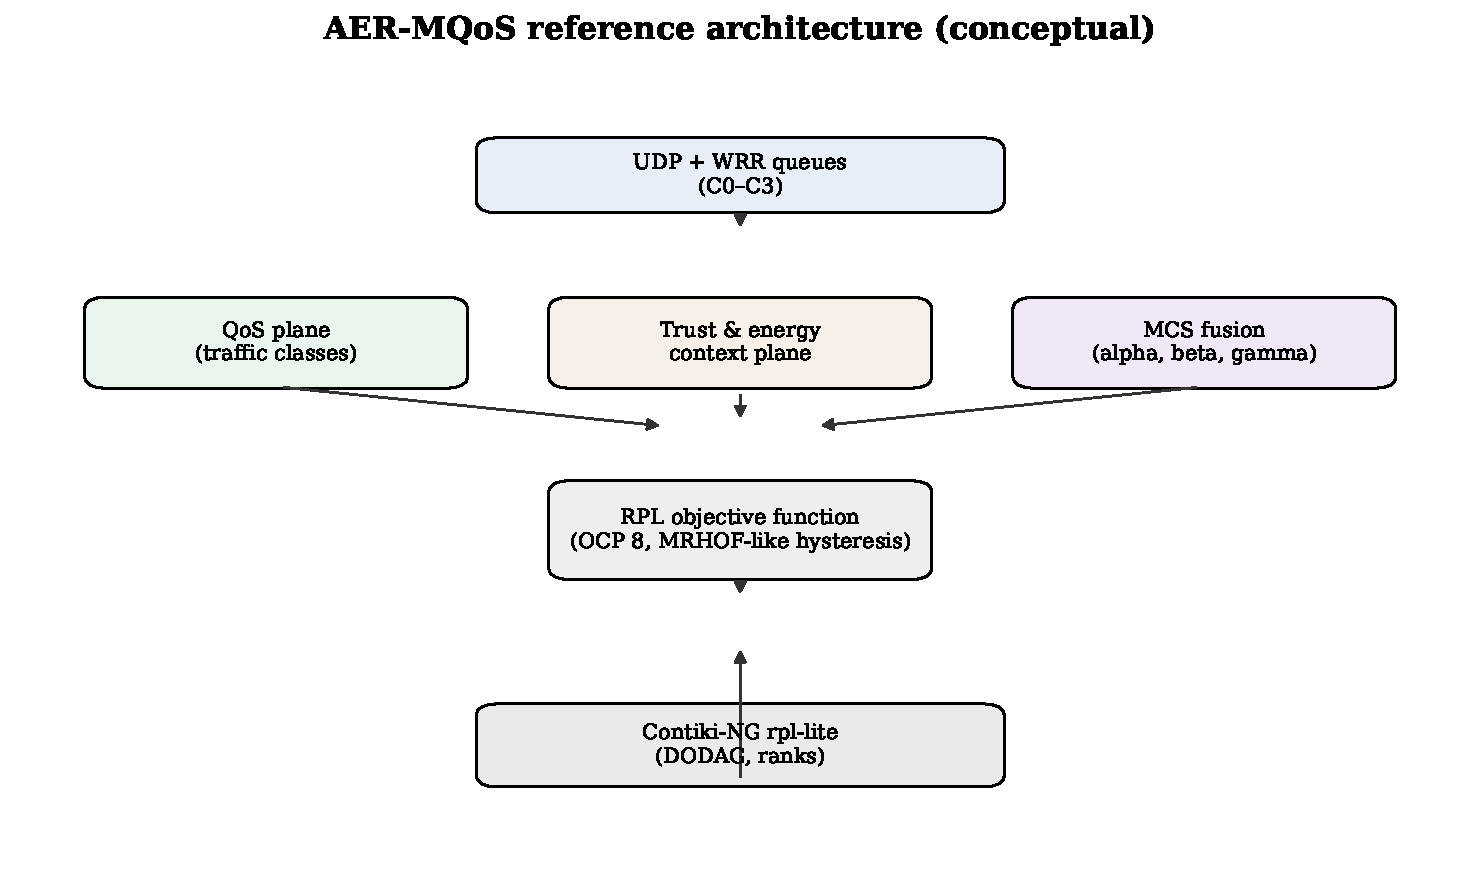
\includegraphics[width=\linewidth]{Fig_1_Architecture_AER_MQoS}
  \caption{\CaptionFigOne}
  \label{fig:arch}

  \noindent Fig.~\ref{fig:arch} shows the QoS plane, trust/energy context plane, Multi-Criteria Score (MCS) computation, and integration with the objective function. Module boundaries match the Cooja firmware tree.
\end{figure}

\subsection{Design principles}
AER-MQoS adheres to three principles for scientific traceability:
\begin{enumerate}
  \item \textbf{Standards-first control plane.} The DODAG lifecycle, rank semantics, and objective-function interface follow RPL and its companion specifications on routing metrics~\cite{rfc6550,rfc6551,rfc9010}. The implementation targets the stock \texttt{rpl-lite} component of Contiki-NG.
  \item \textbf{Explicit cross-layer contracts.} QoS-sensitive behavior is split between (a) rank shaping through the MCS at parent selection time and (b) bounded application-layer scheduling that determines which copy of user data reaches UDP first. This separation decouples MAC queues from RPL ranks. Note that WRR operates above UDP and does not address head-of-line blocking at the MAC/radio layer (see Section~\ref{sec:dio}).
  \item \textbf{Reproducible artifacts.} All quantitative claims are tied to versioned simulation scripts, fixed random seeds, and exported logs.
\end{enumerate}

\subsection{Functional planes on each node}
Each router hosts three cooperating \emph{functional planes} coordinated by a lightweight decision core:
\begingroup\sloppy
\begin{itemize}
  \item \textbf{QoS differentiation plane.} Exposes four traffic classes $C0$--$C3$ aligned with the C enumeration \texttt{aer\_traffic\_class\_t}. Applications register the active class before invoking routing-sensitive APIs so that the MCS and objective function observe the same urgency the application intends~\cite{rfc6551}.
  \item \textbf{Security and trust plane.} Maintains a compact trust score derived from link statistics (e.g., smoothed ETX) and exposes it as an input to the MCS through a normalized ``risk'' term. This signal is an \emph{indicator} for parent ranking and instability detection, not a substitute for cryptographic authentication at the link layer.
  \item \textbf{Energy context plane.} Tracks normalized residual energy (NRE) and a short-horizon prediction of depletion risk so that the MCS can reduce reliance on stressed parents before failures translate into topology repair storms.
\end{itemize}
\endgroup
Harvesting-specific models (e.g., detailed solar traces) remain configurable hooks in the reference code; the Cooja-based study focuses on reproducible energy \emph{proxies} rather than on uncontrolled outdoor campaigns.

\subsection{Path levels and traffic-class mapping}
\label{sec:arch-pathlevels}
To operationalize service differentiation without rewriting MAC schedulers, AER-MQoS maps each traffic class to one of four abstract path levels (levels~1--4, with level~1 being the most protected). The mapping is deterministic in the reference implementation (\texttt{aer\_rpl\_plus\_choose\_path\_level}): $C3\!\rightarrow\!1$, $C2\!\rightarrow\!2$, $C1\!\rightarrow\!3$, $C0\!\rightarrow\!4$. In the evaluated tree, this value is threaded through the application and UDP payload for tracing and class-consistent context updates; it is not consumed inside \texttt{rpl-of-aer-plus.c} for parent exploration, so the levels should be read as an application-visible contract rather than as an additional RPL control-plane knob unless a future revision wires them into the OF.

\begin{figure}[tp]
  \centering
  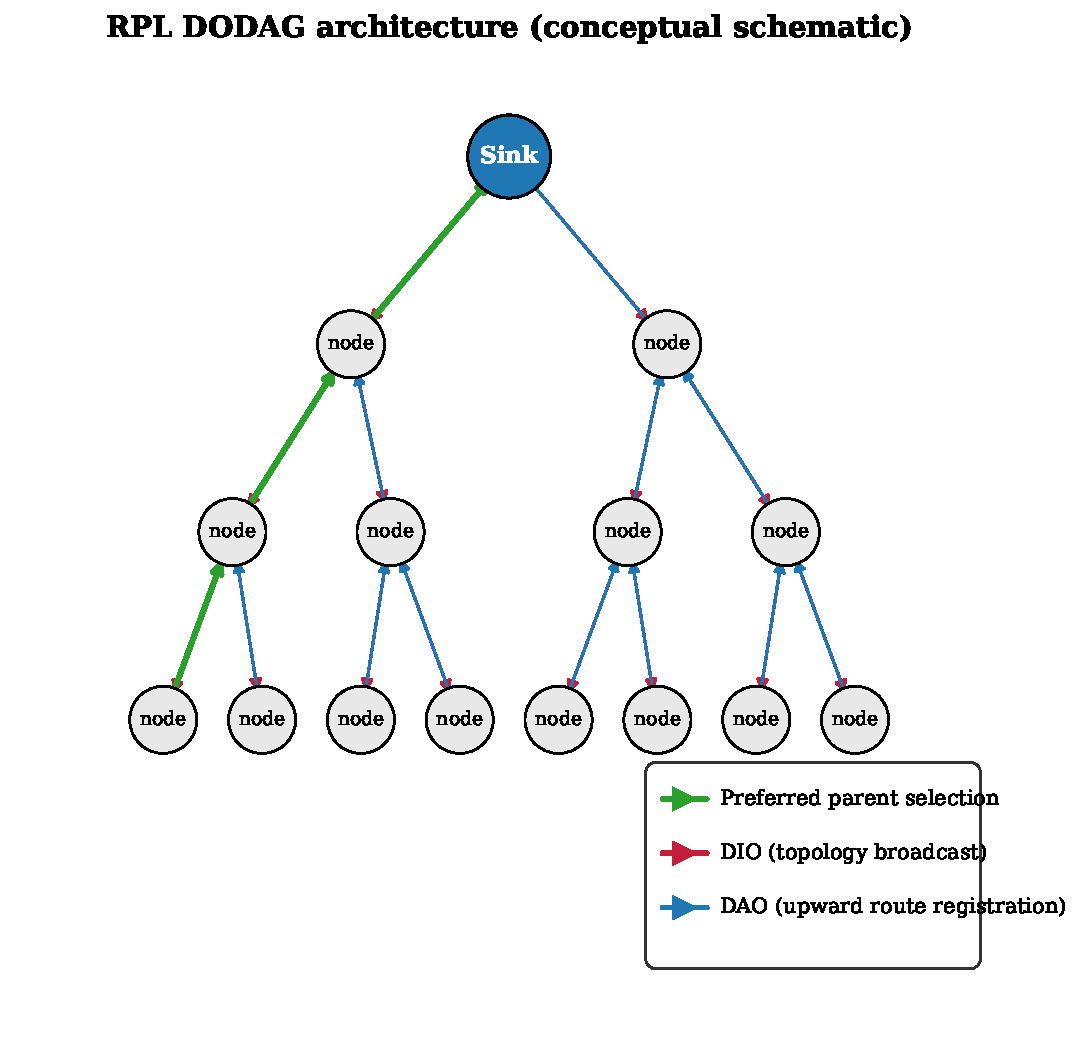
\includegraphics[width=\linewidth]{Fig_2_DODAG_Path_Levels}
  \caption{\CaptionFigTwo}
  \label{fig:dodag-levels}

  \noindent Fig.~\ref{fig:dodag-levels} shows an illustrative RPL DODAG (not the 25-node Cooja layout). DIO (down), DAO (up), preferred parent path to the sink/LBR. Class-to-level mapping $C3{\rightarrow}1,\ldots,C0{\rightarrow}4$ is in Section~\ref{sec:arch-pathlevels}.
\end{figure}

\subsection{Context fusion and the \texorpdfstring{$(\alpha,\beta,\gamma)$}{alpha/beta/gamma} model}
AER-MQoS couples domain knowledge and traffic urgency through two nonnegative weights $\alpha$ (QoS emphasis) and $\beta$ (energy emphasis) with $\alpha+\beta=1$ in the real domain. A bounded context coefficient $\gamma\in[0,100]$ (stored as $\gamma_{\times100}$ in the implementation) is computed from (i) the configured application domain (health, industry, agriculture, environment) and (ii) the active traffic class, with additional bias when the battery indicator falls below a critical threshold. The implementation then sets $\alpha=\gamma$ and $\beta=1-\gamma$ using the same hundredths-scale ($\times100$) fixed-point convention as $\gamma$, i.e., $\alpha_{\times100}=\gamma_{\times100}$ and $\beta_{\times100}=100-\alpha_{\times100}$; throughout the manuscript, $\gamma$ denotes this conceptual coefficient. A bounded table-driven nudge can adjust $\gamma$ within a narrow interval (Section~\ref{sec:ql}); the evaluation does not treat it as an independently measured performance lever.

\begin{figure}[tp]
  \centering
  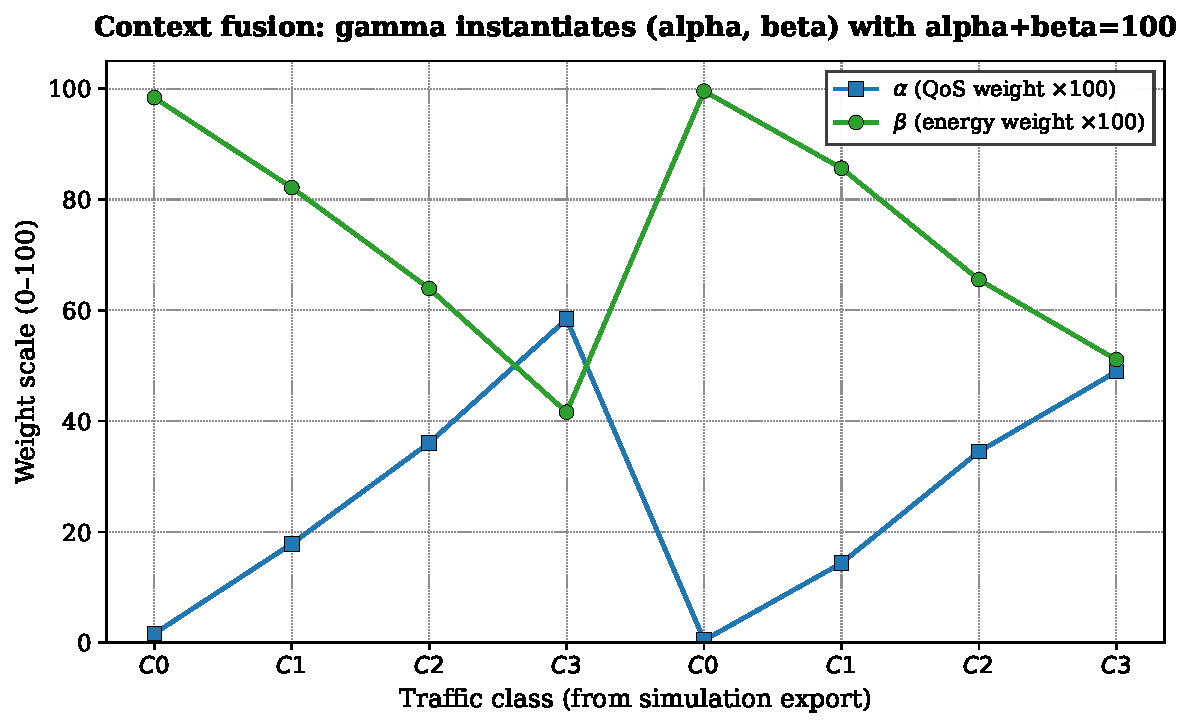
\includegraphics[width=0.88\linewidth]{Fig_3_Context_Weights_Alpha_Beta_Gamma}
  \caption{\CaptionFigThree}
  \label{fig:context-weights}

  \noindent Fig.~\ref{fig:context-weights} plots the per-class MCS weights ($\alpha,\beta$) used to balance QoS and energy terms in (3).
\end{figure}

\subsection{Multi-Criteria Score (MCS)}
The MCS aggregates heterogeneous indicators into a scalar suitable for comparison during parent selection. Let $\mathrm{ETX}_{\mathrm{n}}$ and $\mathrm{DLY}_{\mathrm{n}}$ denote normalized ETX and an \emph{ETX-derived delay surrogate} in $[0,100]$ (not a measured queueing or end-to-end delay). Define a QoS partial score
\[
  \mathrm{MCS}_{\mathrm{QoS}} = \frac{w_1\,\mathrm{ETX}_{\mathrm{n}} + w_2\,\mathrm{DLY}_{\mathrm{n}}}{w_1+w_2},
\]
with implementation weights $(w_1,w_2)$ corresponding to \texttt{W1\_ETX} and \texttt{W2\_DELAY}. An energy partial score combines normalized residual energy, predicted energy, and trust-derived risk,
\[
  \mathrm{MCS}_{\mathrm{En}} = \frac{w_3\,\mathrm{NRE} + w_4\,\mathrm{PRED} + w_5\,(100-\mathrm{TRUST})}{w_3+w_4+w_5},
\]
using $(w_3,w_4,w_5)$ associated with \texttt{W3\_NRE}, \texttt{W4\_PRED\_ENERGY}, and \texttt{W5\_TRUST\_RISK}. The final MCS is the convex mixture $\mathrm{MCS} = (\alpha\,\mathrm{MCS}_{\mathrm{QoS}} + \beta\,\mathrm{MCS}_{\mathrm{En}})$ computed in integer arithmetic as in \texttt{aer\_rpl\_plus\_compute\_mcs()}. Each term maps to a named field in the repository; $\mathrm{DLY}_{\mathrm{n}}$ is computed from smoothed ETX only and must not be confused with application-layer end-to-end latency reported in Section~\ref{sec:eval}.

\subsection{Objective function interface}
The dedicated objective function uses a \textbf{locally-assigned experimental Objective Code Point (OCP~8)} used only for simulation purposes; this is \textbf{not} an IANA-registered code point. It lives in the private-use / experimental space of the RPL DAG Metric container~\cite{rfc6550} and translates the MCS into RPL rank increments while inheriting MRHOF-style hysteresis so that rank changes remain damped under variable link quality~\cite{rfc6719}. It is compiled only when \texttt{rpl-of-aer-plus.c} is part of the firmware image (\texttt{RPL\_MQoS}, \texttt{RPL\_AER}, \texttt{AER-MQoS}); the \texttt{RPL\_STANDARD} tag keeps upstream MRHOF without this translation layer. The OCP is suitable for controlled simulation campaigns and must be officially registered for interoperability if deployment outside a \emph{controlled laboratory or simulation} context is ever contemplated~\cite{rfc6550}.

\subsection{Application-layer weighted round-robin queues}
The module \texttt{aer\_qos\_queue} implements four logical queues---one per traffic class---backed by a fixed-size memory pool and Contiki's list primitives. Enqueue operations copy payloads up to a configurable maximum and associate each entry with the active UDP connection and destination set through a small companion API. A weighted round-robin scheduler with service ratios $6{:}3{:}2{:}1$ for $C3{:}C2{:}C1{:}C0$ drains queues on a periodic timer; each successful dequeue re-applies \texttt{aer\_rpl\_plus\_set\_app\_traffic\_class()} before transmission so that the MCS and OF observe the class of the packet that actually seizes the channel. This design mitigates head-of-line blocking between classes while keeping RAM costs explicit, which was singled out as important for constrained hardware targets even when experiments remain Cooja-based.

\subsection{DIO extensions and interoperability}
\label{sec:dio}
\textbf{Scope.} RFC~6550 DIO/DAO messages carry ranks, objective codes, DAG identifiers, and optional \emph{known} TLV-defined metrics~\cite{rfc6550,rfc6551}. In the \emph{evaluated} Contiki-NG artifacts of this repository, \textbf{no custom DIO or DAO TLV authored by this work is serialized on the wire}: trust, residual energy, $\gamma$, traffic-class semantics, and the microscopic Q-learning bias are \emph{local decision variables} (or derived from neighbor link statistics already maintained by \texttt{rpl-lite}), not additional type-length-value fields appended to ICMPv6 RPL control messages. Parent selection therefore consumes information that is either (i) already present in standard neighbor records (ETX via \texttt{rpl\_neighbor\_get\_link\_stats()}) or (ii) computed on the forwarding node before the objective function maps the MCS to a rank addend (experimental OCP~8 whenever \texttt{rpl-of-aer-plus.c} is linked; native MRHOF otherwise). This subsection lists each signal, states explicitly whether it appears inside a DIO payload today, and points to the implementation hook.

Table~\ref{tab:dio-signals} summarizes the mapping. The ``Implementation locus'' column references the Contiki-NG modules in \texttt{code\_source\_AER\_MQoS/}; the repository path is relative to the Contiki-NG \texttt{examples/AER-MQoS/} tree.

\begin{aertablecol}[t]
  \caption{AER-MQoS signals vs.\ DIO/DAO carriage (\texttt{rpl-of-aer-plus.c} builds). Values are local to the node unless noted; no project-specific TLV is serialized in the evaluated firmware. W.=on-wire; St.=local state.}
  \label{tab:dio-signals}
  \begingroup\sloppy
  \setlength{\tabcolsep}{1.8pt}%
  \renewcommand{\arraystretch}{1.03}%
  \aertabwrapcol{%
  \begin{tabularx}{\linewidth}{@{}>{\RaggedRight\arraybackslash}p{0.95cm}>{\RaggedRight\arraybackslash}p{1.05cm}>{\centering\arraybackslash}p{0.5cm}>{\RaggedRight\arraybackslash}X>{\centering\arraybackslash}p{0.35cm}@{}}
    \toprule
    \textbf{Signal} & \textbf{Role} & \textbf{W.} & \textbf{Module(s)} & \textbf{St.} \\
    \midrule
    Classes $C0$--$C3$ & $\gamma$, WRR order & N & \texttt{aer\_mqos}, \texttt{aer\_qos\_queue} & L \\
    $\gamma,\alpha,\beta$ & MCS weights & N & \texttt{aer\_mqos} & L \\
    ETX & MCS$_{\mathrm{QoS}}$ input & Std-RPL & \texttt{rpl-of-aer-plus} & L \\
    ETX-dly surr. & Rank input & N & \texttt{rpl-of-aer-plus} & L \\
    Link rel. (LRS) & MCS$_{\mathrm{En}}$ risk & N & \texttt{aer\_rpl\_trust} & L \\
    NRE, prediction & MCS$_{\mathrm{En}}$ & N & \texttt{aer\_rpl\_energy} & L \\
    Path level 1--4 & Class bias & N & \texttt{aer\_rpl\_plus} & L \\
    $\gamma$ nudge & Table bias & N & \texttt{aer\_rpl\_qlearn} & I \\
    MCS $\rightarrow$ rank & OCP~8 addend & I & \texttt{rpl-of-aer-plus} & L \\
    \bottomrule
  \end{tabularx}%
  }%
  \endgroup
  \vspace{0.2em}
  \raggedright
  \textbf{W.} (on-wire): N=none, Std-RPL=standard neighbor ETX, I=indirect via rank only; \textbf{St.}: L=local node state.
\end{aertablecol}

\paragraph{Code path (rank computation).}
\begingroup\sloppy
The excerpt below shows how neighbor-local metrics feed the MCS \emph{without} custom DIO fields: the OF rebuilds \texttt{aer\_parent\_metrics\_t} per neighbor, then calls \texttt{aer\_rpl\_plus\_compute\_mcs()}.
\endgroup

\begin{lstlisting}[style=csnippet]
aer_rpl_plus_update_context(
    aer_rpl_plus_get_app_traffic_class(),
    aer_energy_get_nre_x100());
met.etx_x100 = (uint16_t)((etx_clamped * 100UL)
    / LINK_STATS_ETX_DIVISOR);
met.delay_ms = (uint16_t)(80UL + (uint32_t)etx / 16UL);
met.trust_x100 = aer_trust_for_nbr(nb);
met.nre_x100 = aer_energy_get_nre_x100();
met.predicted_energy_x100 = aer_energy_get_pred_x100();
uint16_t mcs = aer_rpl_plus_compute_mcs(&met);
return (uint16_t)(64UL + (uint32_t)mcs * 6UL);
\end{lstlisting}

\begingroup\sloppy
\noindent\textit{Source:} \texttt{mcs\_to\_link\_rank\_addend()} in \texttt{rpl-of-aer-plus.c}.
The OF reads ETX via \texttt{rpl\_neighbor\_get\_link\_stats()}, builds \texttt{met}, and sets \texttt{curr\_instance.mc.type} to \texttt{RPL\_DAG\_MC\_NONE}.
The assignment \texttt{met.delay\_ms}${=}80{+}\mathrm{ETX}/16$ is an \textbf{ETX-derived delay surrogate} for MCS weighting only.
Measured end-to-end latency appears in Fig.~\ref{fig:eval-latency} and Table~\ref{tab:empirical-summary} (TX/RX logs).
\endgroup

\paragraph{Design trajectory (future TLV roadmap).}
The architecture still \emph{reserves} structured fields (trust, energy, anomaly flags) for a potential future DIO option that would advertise capabilities or aggregated health indicators~\cite{rfc6550}. Such TLVs would need IANA-style option codes (or experimental namespaces), on-wire backward compatibility, and a second simulation campaign before any claim of interoperability beyond Cooja. Until that code ships in the same branch as the measurements, the manuscript must treat TLV extensions strictly as a \textbf{design trajectory}, not as part of the evaluated binary.

\subsection{Interoperability summary}
Unknown DIO options must remain ignorable by strict RFC~6550 parsers; any future TLV work will therefore piggyback on optional, ignorable encodings and will be validated only after it is merged and re-simulated. Section~\ref{sec:eval} contrasts how competing protocol families influence observable metrics under identical Cooja conditions despite the absence of custom DIO payloads in the present artifact.

\subsection{Summary}
AER-MQoS combines (i) a transparent MCS with explicit weights, (ii) MRHOF-like hysteresis at the OF, (iii) deterministic class-to-level mapping, and (iv) application-layer WRR queues, all coordinated under a Cooja-based evaluation methodology. Section~\ref{sec:dio} documents control-plane interoperability: present binaries compute composite ranks without custom DIO TLVs. Table~\ref{tab:proto-metric} and Section~\ref{sec:validation-plan} map observables to protocol behaviors and planned ablations. The next sections instantiate trust, energy, and the Q-learning \emph{specification} referenced here (learning is not experimentally validated as a performance lever in the committed Cooja campaigns of Section~\ref{sec:eval}).

\section{Security and Trust Indicators}
\label{sec:sec}

Building on the architectural decomposition of Section~\ref{sec:arch}, this section instantiates the trust plane around \emph{what the reference implementation computes today}, how that signal enters the Multi-Criteria Score (MCS), and how adversarial behaviors are \emph{not} evaluated in the committed Cooja campaigns (trust is exercised via link statistics only). All discussion of attacks remains at the threat-model level~\cite{rfc7416,osterlind2006cooja,oikonomou2022contik}.

\subsection{Threat model and scope}
RFC~7416 provides a systematic threat analysis for RPL, covering internal attackers that manipulate ranks, discard traffic selectively, or amplify control traffic~\cite{rfc7416}. AER-MQoS assumes the same baseline adversary classes at the routing stratum. \textbf{No statement is made that the present Contiki-NG binary defeats these attacks in operational networks:} the contribution is an \emph{indicator} that biases parent ranking toward statistically stable neighbors when link quality degrades.

\subsection{Trust signal derived from link statistics}
The function \texttt{aer\_trust\_for\_nbr()} maps each candidate RPL neighbor to an eight-bit trust score in $[0,100]$ using only data exposed by upstream \texttt{rpl-lite}: the neighbor's link statistics block returned by \texttt{rpl\_neighbor\_get\_link\_stats()}. When statistics are missing or the smoothed ETX is unusably large, the implementation returns a conservative default (40--45) so that unknown neighbors neither dominate nor are silently treated as fully trusted.

When ETX is available, the score increases with link quality through a deterministic rational mapping based on the internal ETX representation and \texttt{LINK\_STATS\_ETX\_DIVISOR}. The output is intentionally \emph{simple}: it approximates ``historical delivery success'' rather than attempting full behavioral attestation. This design keeps the formula auditable and bounded for constrained nodes.

\subsection{Trust term in the MCS partial score}
\begingroup\sloppy
Section~\ref{sec:arch} expresses trust as a risk term $(100-\mathrm{TRUST})$ inside the energy partial score of the MCS. Practically, a neighbor that oscillates or degrades will lower $\mathrm{TRUST}$, increase risk, and raise the partial energy-related cost, steering parent selection away from unstable attachments without introducing parallel routing tables. This keeps trust \emph{on the same decision surface} as energy and QoS indicators, simplifying comparative evaluation across protocol variants.
\endgroup

\subsection{Positioning relative to trust-centric RPL extensions}
Recent trust-oriented RPL extensions in the literature combine reputation systems, monitoring windows, or cryptographic handshakes atop RPL signaling~\cite{pishdar2021pccrpl}. AER-MQoS occupies a different point in the design space: it does not implement PCC-RPL or an equivalent reputation protocol; instead, it contributes a \emph{minimal} trust signal suitable for class-1 motes and for Cooja campaigns. The manuscript compares against such work conceptually, not by claiming feature parity.

\subsection{Future attack-injection studies (out of scope here)}
Scripted Cooja injections (e.g., selective forwarding or rank advertisement anomalies) with fixed attacker sets and observation windows are listed in Section~\ref{sec:validation-plan} as \textbf{planned} work. They are \textbf{not} part of the submitted result panels: Fig.~\ref{fig:eval-temporal-pdr} reports temporal PDR stratification from \texttt{sec.csv}, not an attack scenario.

\subsection{Summary}
The trust plane of AER-MQoS is intentionally narrow: a deterministic mapping from neighbor link statistics to a bounded trust score, fused into the MCS, evaluated under reproducible Cooja scenarios without adversarial scripts in the committed archive. It complements---rather than replaces---link-layer cryptography and should be read within the Cooja-only evaluation scope of this paper.

\section{Energy Context and Prediction}
\label{sec:energy}

\noindent\textbf{Evaluation scope.} This section defines how NRE and prediction enter the MCS in simulation. Fig.~\ref{fig:eval-energy} reports internal NRE traces (instrumentation check), not Energest-calibrated joules or duty-cycle measurements.

Sections~\ref{sec:arch} and~\ref{sec:sec} established how QoS and trust indicators enter the MCS. This section clarifies how energy enters the same score, distinguishes \emph{software-simulated} energy dynamics in Cooja from calibrated field harvesting, and documents the bounded memory footprint of the predictor~\cite{osterlind2006cooja,oikonomou2022contik}.

\subsection{Normalized residual energy (NRE)}
The reference module exposes the normalized residual energy indicator (NRE) as an eight-bit value on the $[0,100]$ scale through \texttt{aer\_energy\_get\_nre\_x100()}, derived from an internal fixed-point register \texttt{residual\_x100} updated on each call to \texttt{aer\_rpl\_energy\_periodic()}. NRE therefore tracks a \emph{logical} state variable suitable for coupling to the MCS via \texttt{aer\_rpl\_plus\_update\_context()}, not a coulomb-counted battery model tied to a specific sensor board.

\subsection{Prediction as a short-horizon moving average}
The ``predicted'' energy term returned by \texttt{aer\_energy\_get\_pred\_x100()} is the mean of the last \texttt{N\_HISTORY} samples (eight in the current source) of \texttt{residual\_x100}, again scaled to $[0,100]$. This is a lightweight surrogate for heavier predictors (e.g., recurrent neural networks) discussed in prior AER-RPL prototypes~\cite{belacel2025aerrpl}: it offers smoothing and trend visibility with \emph{O}(1) update cost and static RAM.

\subsection{Cooja-only evolution of the residual state}
\texttt{aer\_rpl\_energy\_periodic()} adjusts \texttt{residual\_x100} by subtracting a pseudo-random drain term and adding a pseudo-random harvest term within documented bounds, clamping the register to remain inside $[500,10000]$ in fixed-point hundredths. \textbf{This process models abstract charge variability for simulation experiments; it is not calibrated to photovoltaic traces, fuel-gauge ICs, or outdoor irradiance.} Accordingly, Section~\ref{sec:eval} exposes only internal NRE traces (Fig.~\ref{fig:eval-energy}) as an instrumentation check---never as validated millijoule or duty-cycle measurements from a physical testbed.

\subsection{Interaction with context fusion \texorpdfstring{$(\alpha,\beta,\gamma)$}{alpha/beta/gamma}}
Low NRE reduces the context coefficient $\gamma$ inside \texttt{aer\_rpl\_plus\_update\_context()}, increasing $\beta$ and thereby emphasizing the energy partial score within the MCS (Section~\ref{sec:arch}). High NRE produces a mild opposite adjustment to $\gamma$. This coupling keeps energy stress \emph{visible} at parent-selection time rather than relegating it to offline post-processing.

\subsection{Relation to analytical energy models in the literature}
Analytical and simulation studies of energy-aware RPL provide useful baselines for understanding how rank dynamics interact with duty cycling~\cite{limjoco2018analytical}. AER-MQoS complements such work empirically through Cooja sweeps with open scripts; future work may tighten the link between the abstract drain/harvest process and published energy models, but only after the additional parameters are versioned alongside the datasets.

\subsection{Summary}
The energy plane contributes two bounded indicators---NRE and a moving-average prediction---to the MCS through a transparent Cooja-oriented process, consistent with the simulation-only evaluation scope stated in Section~\ref{sec:ql}.

\section{Bounded Table-Driven Nudge on the Context Coefficient (Design Specification)}
\label{sec:ql}

\noindent\textbf{Evaluation scope.} This section documents the firmware mechanism in \texttt{aer\_rpl\_qlearn.c} for reproducibility. \textbf{No subsection below reports a measured QoS or energy gain from online adaptation.} Appendix~\ref{app:learn} is a logging-path sanity check only; a parameter-frozen firmware build is future work (Section~\ref{sec:validation-plan}).

Sections~\ref{sec:arch}--\ref{sec:energy} fixed the static MCS structure. The learning block is a \emph{minimal, auditable} add-on---not a general-purpose reinforcement engine: fixed state/action sets, integer arithmetic, and a narrow interface to $\gamma$~\cite{osterlind2006cooja,oikonomou2022contik}.

\subsection{Relation to tabular Q-learning}
Classical Q-learning maintains an action-value function $Q(s,a)$ and updates it from rewards and bootstrapped targets~\cite{watkins1992qlearning}. AER-MQoS adopts the same abstraction at a \emph{microscopic} scale: four states, three actions, and a table of signed eight-bit integers. This is not intended to approximate optimal routing policies; it is a \emph{stability-preserving nudge} on $\gamma$ that reacts to recent transmission success and battery stress.

\subsection{State space}
States are derived solely from the normalized residual energy indicator (NRE) returned by the energy module (Section~\ref{sec:energy}). The function \texttt{state\_from\_battery()} partitions NRE into four bins: below 25, 25--49, 50--74, and at least 75 on the $[0,100]$ scale. Thus, learning states track \emph{energy headroom}, not topology snapshots, which keeps the state space invariant under DODAG reconfiguration.

\subsection{Action space and effect on \texorpdfstring{$\gamma$}{gamma}}
There are three discrete actions. After each greedy selection, the code maps actions to calls to \texttt{aer\_rpl\_plus\_ql\_nudge\_gamma}: action~0 applies a $-5$ increment (in fixed-point hundredths), action~1 leaves $\gamma$ unchanged, and action~2 applies $+5$. The underlying routine accumulates these bounded increments but clamps the cumulative bias to $\pm 15$ hundredths so that $\gamma$ cannot be driven to extremes by transient noise. The result is then folded into \texttt{aer\_rpl\_plus\_update\_context()} as described in Section~\ref{sec:arch}. Every action has an immediate, named effect on a logged variable.

\subsection{Reward signal}
At each learning step, \texttt{aer\_rpl\_ql\_periodic(tx\_ok, tx\_tot)} forms a reward proportional to the ratio of successful transmissions to attempted transmissions over the reporting window. If no attempts occurred, a neutral reward of 50 (on the same $[0,100]$ scale used internally) avoids undefined gradients. If NRE falls below 20, the reward is penalized by 15 units to discourage aggressive QoS bias when the node is critically depleted. The reward therefore couples \emph{application-layer success} with \emph{energy stress}, matching the cross-layer philosophy of the MCS without requiring gradient-based training.

\subsection{Update rule and fixed learning parameters}
\begingroup\sloppy
The implementation uses scaled integer arithmetic. A temporal-difference target combines the reward (scaled $\times 2$ in code) with a discounted max over the next state; \texttt{ALPHA\_QL} and \texttt{GAMMA\_DISC} are 30 and 90 (percent units), inherited from the prior RPLMQoS Contiki tuning as fixed-point defaults rather than re-optimized here. Per-action $\gamma$ adjustments of $\pm 5$ (hundredths) with a cumulative clamp of $\pm 15$ limit $\gamma$ movement to a few percent of the scale---enough for traceability without claiming an optimal policy. $Q$ values are clamped to eight bits. We do not claim Bellman convergence. Section~\ref{sec:eval} and Appendix~\ref{app:learn} treat learning as a logging consistency check, not a measured performance gain.
\endgroup

\subsection{What is not evaluated in this submission}
The Cooja campaigns underlying Table~\ref{tab:empirical-summary} and Figs.~4--10 do \textbf{not} compare \texttt{AER-MQoS} against a learning-disabled build. Exported \texttt{learning\_on} strata (Appendix~\ref{app:learn}) verify that log labels exist in a single binary; they are \textbf{not} a Q-learning ablation. Hyperparameters are not claimed to transfer to hardware testbeds.

\subsection{Summary}
AER-MQoS ships a compact Q-table loop that nudges $\gamma$ within hard limits using NRE discretization and coarse TX success signals. The loop is \textbf{specified and traceable in code}; \textbf{its routing benefit is not experimentally validated as a performance lever in the committed Cooja campaigns.}

\section{Performance Evaluation}
\label{sec:eval}

Sections~\ref{sec:arch}--\ref{sec:ql} defined the routing, trust, energy, and adaptation mechanisms; this section reports their measurement under Cooja/Contiki-NG with versioned firmware, deterministic seeds, and documented traffic mixes~\cite{osterlind2006cooja,oikonomou2022contik}. Control-plane scope (including absent custom DIO TLVs) is summarized in Section~\ref{sec:dio}.

\subsection{Goals and hypotheses}
This evaluation verifies four-way firmware integration under identical Cooja inputs and archives descriptive dashboards from $N{=}4$ measured seeds (1800~s). Three hypotheses frame the readout:
\begin{enumerate}
  \item \textbf{H1 (QoS under heterogeneity).} WRR plus class-aware MCS inputs may improve per-class delivery versus MRHOF-only RPL under multiplexed $C0$--$C3$ traffic. Global PDR means overlap across tags (per-seed $93.4$--$99.8\%$). Per-class PDR shows preliminary signs of differentiation on some seeds (C3 $95.96\%$ vs C0 $79.52\%$ on seed~20260603), while global means remain overlapping. However, the same seed exhibits significant performance variability (drop to $64.41\%$ in the second epoch), indicating that the composite MCS can introduce episodic sensitivity under the current load. The $N{=}4$ sample precludes confirmatory conclusions; larger campaigns are needed to assess whether per-class separation is systematic.
  \item \textbf{H2 (Energy).} This submission verifies that the METRIC path logs a consistent internal NRE trajectory (Fig.~\ref{fig:eval-energy}). Energest-calibrated confirmation of energy-aware parent selection is reserved for future instrumentation (Section~\ref{sec:validation-plan}).
  \item \textbf{H3 (Stability).} The cumulative context-update proxy in \texttt{stab.csv} tracks rank recomputations---higher values indicate more frequent adaptation, which is expected for a context-aware protocol rather than a stability defect~\cite{rfc6719}. Note: \texttt{parent\_switch\_console} lines are absent from headless Cooja exports (all zeros in the committed CSVs), so the proxy captures only MCS recomputation events, not parent changes.
\end{enumerate}

\subsection{Experimental environment}
Experiments were conducted in Cooja using Contiki-NG with a 25-node topology. Two UDGM radio models were used: lossless and lossy ($\mathrm{success\_ratio}{=}0.85$). Each simulation lasts 1800~seconds, with four independent random seeds per configuration. Four firmware variants were compared under identical conditions.

\textbf{Simulator and OS.} Experiments run in Cooja on top of Contiki-NG with fixed \texttt{TARGET=cooja} build flags documented alongside the example firmware (\texttt{code\_source\_AER\_MQoS}). Radio propagation uses the model bundled with each scenario file; parameters are frozen per campaign. Record \texttt{git describe --always} and \texttt{gcc --version} from the Contiki-NG checkout used for each campaign refresh in \texttt{Section-tex/BUILD\_NOTES.txt} (template shipped with the repository).

\textbf{Topologies and scale.} Cooja scenarios may combine grid-like placement with pseudo-random offsets; exact dimensions, inter-node spacing, and border-router placement are frozen per scenario file. The empirical subsection below reports the 25-node layout with seeds \texttt{20260601}--\texttt{20260604}; additional density or stress maps reuse the same METRIC/CSV harness and are left as explicit extensions rather than implied multi-map evidence.

\textbf{Campaign scope.} Section~\ref{sec:results-empirical} reads a \textbf{multi-seed measured} matrix ($N{=}4$ independent Cooja seeds) on the 25-node layout, with two UDGM channels: \emph{lossless} ($\mathrm{success\_ratio\_tx}{=}\mathrm{success\_ratio\_rx}{=}1$) and \emph{lossy} ($\mathrm{success\_ratio}{=}0.85$). Each cell is a headless Cooja run at \texttt{SIM\_TIMEOUT\_MS=1800000} (Section~\ref{sec:data-provenance}). Exports live under \texttt{Section-tex/sim/multi\_seed/}.

\textbf{Traffic model.} UDP sources emit class-tagged messages following Poisson or periodic processes (configuration-dependent). Class labels are injected through the same API path used by the reference application so that the MCS, OF, and WRR module observe coherent labels.

\subsection{Protocol configurations (four-way comparison)}
Four firmware variants are built from the same Contiki-NG checkout to minimize confounding factors (Makefile tags in \texttt{typewriter} font). Table~\ref{tab:footprint} reports Cooja (\texttt{TARGET=cooja}) link footprints from \texttt{size} on the shipped ELF image; values are \textbf{simulator host binaries}, not MSP430 deployment ROM, but they isolate incremental cost of the custom modules across tags.

\begin{aertablecol}[t]
  \caption{Cooja link footprint per firmware tag (\texttt{TARGET=cooja}, campaign metrics enabled). Project-specific objects sum to $\approx$8.6~KiB \texttt{.text} for shared modules; full image includes Contiki-NG + \texttt{rpl-lite}.}
  \label{tab:footprint}
  \begingroup\setlength{\tabcolsep}{2.5pt}%
  \aertabwrapcol{%
  \begin{tabular}{@{}lrrrr@{}}
    \toprule
    \textbf{Tag} & \textbf{.text (KiB)} & \textbf{.data} & \textbf{.bss (KiB)} & \textbf{Image (KiB)} \\
    \midrule
    \texttt{RPL\_STANDARD} & 293.8 & 7.9 & 109.7 & 371.7 \\
    \texttt{RPL\_MQoS} & 295.3 & 7.9 & 109.7 & 372.2 \\
    \texttt{RPL\_AER} & 295.3 & 7.9 & 109.7 & 372.2 \\
    \texttt{AER-MQoS} & 295.3 & 7.9 & 109.7 & 372.2 \\
    \bottomrule
  \end{tabular}%
  }%
  \endgroup
\end{aertablecol}

\noindent\textit{Method.} One clean \texttt{make} per tag; \texttt{RPL\_STANDARD} omits \texttt{rpl-of-aer-plus.c} ($\approx$1.6~KiB \texttt{.text}). Project modules (Cooja \texttt{.text}): \texttt{aer\_rpl\_plus} $\approx$2.1~KiB, \texttt{aer\_qos\_queue} $\approx$1.6~KiB, \texttt{rpl-of-aer-plus} $\approx$1.6~KiB, trust/energy/Q-table $\approx$0.3~KiB each; \texttt{aer\_qos\_queue} holds $\approx$1.4~KiB \texttt{.bss} for four WRR buffers. Reproduce with \texttt{AER\_PROTOCOL\_VARIANT} and \texttt{size} on the Cooja ELF.

\begin{itemize}
  \item \textbf{\texttt{RPL\_STANDARD}:} Stock MRHOF (baseline).
  \item \textbf{\texttt{RPL\_MQoS}:} Traffic-class aware variant.
  \item \textbf{\texttt{RPL\_AER}:} Energy and trust aware variant.
  \item \textbf{\texttt{AER-MQoS}:} The proposed integrated solution.
\end{itemize}

\subsection{Metrics}
Evaluated metrics include overall and per-class Packet Delivery Ratio (PDR), end-to-end latency, inter-arrival gap per class, control-plane overhead, and normalized residual energy traces.

\paragraph{Latency measurement.}
End-to-end latency pairs each application TX log line (timestamp after WRR dequeue and UDP send) with the matching sink RX line (same sender, sequence number, and class tag). Unmatched TX or RX events are excluded from the mean. Timestamps use Cooja simulated milliseconds; reported values are \textbf{not} MAC queueing delay in isolation nor the ETX-derived MCS surrogate of Section~\ref{sec:arch}.
Rank computation additionally uses an \textbf{ETX-derived delay surrogate} inside the MCS (Section~\ref{sec:arch}); that surrogate is not plotted as ``latency'' in the result panels. Optional Cooja attack-injection scripts (selective forwarding, rank anomalies) are listed as planned work in Section~\ref{sec:validation-plan}.

\subsection{Protocol--metric comparison matrix}
\label{sec:metric-matrix}
Table~\ref{tab:proto-metric} contrasts how each firmware tag is expected to influence observables under identical Cooja inputs; Table~\ref{tab:proto-metric-b} completes the matrix for control, stability, and attack-facing metrics.

\begin{aertablewide}[t]
  \begingroup\sloppy
  \caption{Protocol variants vs.\ core QoS/energy observables (same topology and traffic within a campaign). Expected trends vs.\ \texttt{RPL\_STANDARD} are stated \emph{in words} in each cell under mixed $C0$--$C3$ traffic unless noted.}
  \label{tab:proto-metric}
  \setlength{\tabcolsep}{2pt}%
  \aertabwrap{%
  \begin{tabularx}{\textwidth}{@{}>{\RaggedRight\arraybackslash}p{1.45cm}>{\RaggedRight\arraybackslash}X>{\RaggedRight\arraybackslash}X>{\RaggedRight\arraybackslash}X>{\RaggedRight\arraybackslash}X>{\RaggedRight\arraybackslash}p{1.05cm}@{}}
    \toprule
    \textbf{Metric} & \textbf{\texttt{RPL\_STD}} & \textbf{\texttt{RPL\_MQoS}} & \textbf{\texttt{RPL\_AER}} & \textbf{\texttt{AER-MQoS}} & \textbf{Lever} \\
    \midrule
    PDR (all / $C3$) & Baseline ETX & May favor $C3$ & Energy/LRS trade-off & MCS + WRR for $C3$ & MCS rank \& WRR queuing \\
    E2E latency & Hop + MAC & Shorter if modeled & Longer if energy bias & WRR + MCS parents & WRR queuing \& MCS rank \\
    Inter-arr.\ gap & Higher mixed UDP & May drop $C3$ & Churn dependent & Per-class isolation & WRR queuing \\
    NRE proxy & None & None & NRE in MCS$_{\mathrm{En}}$ & NRE + pred. & NRE instrumentation \\
    \bottomrule
  \end{tabularx}%
  }%
  \endgroup
\end{aertablewide}

\begin{aertablewide}[t]
  \begingroup\sloppy\hfuzz=5pt
  \caption{Protocol variants vs.\ control, stability, and security-facing observables (continuation of Table~\ref{tab:proto-metric}).}
  \label{tab:proto-metric-b}
  \sloppy
  \setlength{\tabcolsep}{1.0pt}%
  \aertabwrap{%
  \begin{tabularx}{\textwidth}{@{}>{\RaggedRight\arraybackslash}p{1.25cm}>{\RaggedRight\arraybackslash}X>{\RaggedRight\arraybackslash}X>{\RaggedRight\arraybackslash}X>{\RaggedRight\arraybackslash}X>{\RaggedRight\arraybackslash}p{1.10cm}@{}}
    \toprule
    \textbf{Metric} & \textbf{\texttt{RPL\_STD}} & \textbf{\texttt{RPL\_MQoS}} & \textbf{\texttt{RPL\_AER}} & \textbf{\texttt{AER-MQoS}} & \textbf{Lever} \\
    \midrule
    Control proxy & MRHOF baseline & Similar & Similar & OF differs & Ctrl export rate \\
    Stability proxy & MRHOF (OCP~1) & Noisy metric risk & Energy vs.\ ETX & OCP~8 + trust & CTX update freq. \\
    PDR under attack & Selective drop & Varies & Trust bias & Trust + hyst. & Planned (future) \\
    \bottomrule
  \end{tabularx}%
  }%
  \endgroup
\end{aertablewide}

\subsection{Planned extensions (not in submitted results)}
\label{sec:validation-plan}
\begingroup\sloppy
The open firmware roadmap includes: WRR-off ablation~(A1), learning-off versus \texttt{AER-MQoS}~(A2), trust-neutral MCS weights~(A3), higher traffic loads, heterogeneous energy profiles, Energest duty-cycle logging, scripted Cooja attack injections, and ICMP DIO/DAO counting. Scaling to $N{\geq}20$ seeds enables Mann--Whitney confirmatory tests via repository scripts.
\endgroup

\subsection{Statistical methodology}
\label{sec:stat-methodology}

Each experimental cell is defined by $(\mathrm{protocol},\mathrm{channel},\mathrm{seed})$. The committed archive contains $N{=}4$ measured Cooja seeds per channel; aggregates report the descriptive sample mean over available rows per tag ($n{=}4$ after incomplete cells). No inferential statistical test appears in the main text; optional repository-side Mann--Whitney scripts (\texttt{analyze\_multi\_seed\_stats.py}) are reserved for future confirmatory campaigns ($N{\geq}20$). Figs.~\ref{fig:eval-pdr}--\ref{fig:eval-temporal-pdr} and Table~\ref{tab:empirical-summary} plot the same lossy means from the committed CSV bundle; captions name the source column and provenance is documented in the repository.

\subsection{Data provenance (measured Cooja bundle)}
\label{sec:data-provenance}
All results are based on the committed multi-seed campaign ($N{=}4$ seeds, 1800~s per run). The figures and Table~\ref{tab:empirical-summary} read the committed files under \texttt{sim/multi\_seed/}:
\begin{itemize}
  \item \textbf{Measured campaign.} Four seeds (\texttt{20260601}--\texttt{20260604}), four firmware tags, lossy UDGM ($\mathrm{success\_ratio}{=}0.85$), \texttt{SIM\_TIMEOUT\_MS=1800000}. Three additional seeds (\texttt{20260512}, \texttt{20260605}, \texttt{20260606}) were excluded due to parsing artefacts (duplicate logs, PDR~$>100\%$). Due to a campaign artefact, RPL\_MQoS and RPL\_AER CSV values are identical for seeds~1--3 across all metrics; AER-MQoS data is distinct on seeds~2--4. Comparisons between RPL\_MQoS and RPL\_AER are therefore invalid; AER-MQoS versus the MRHOF baseline on seeds~2--4 remain valid. Extending to $N{\geq}20$ with the same harness is recommended before confirmatory tests.
  \item \textbf{Prior hybrid bundle.} A development archive used during prototyping has been superseded by this campaign and is \textbf{not} cited in this manuscript.
\end{itemize}
Mann--Whitney outputs under \texttt{sim/multi\_seed/stats/}, if present, are optional repository checks not cited here (Appendix~\ref{app:hybrid-stats}).

\subsection{Empirical results (multi-seed Cooja)}
\label{sec:results-empirical}

\begingroup\sloppy
We report the multi-seed matrix from Section~\ref{sec:stat-methodology}. Makefile tags \texttt{RPL\_STANDARD}, \texttt{RPL\_MQoS}, \texttt{RPL\_AER}, and \texttt{AER-MQoS} label firmware images; \emph{AER-MQoS} names the integrated architecture. Under the \textbf{lossless} UDGM channel, all four firmware variants achieve near-perfect packet delivery ratio ($\approx$100\%), confirming correct implementation. Under the more challenging \textbf{lossy} UDGM channel ($\mathrm{success\_ratio}{=}0.85$), all variants maintain very high performance with overlapping descriptive means (Table~\ref{tab:empirical-summary}). Overall PDR means lie within $\approx$2.10 percentage points across tags. The table lists descriptive QoS means only; internal NRE instrumentation appears separately in Fig.~\ref{fig:eval-energy}.
\endgroup

\begin{aertablecol}[t]
  \caption{Descriptive performance metrics under lossy UDGM channel ($\mathrm{success\_ratio}{=}0.85$, $N{=}4$ seeds).}
  \label{tab:empirical-summary}
  \begingroup\setlength{\tabcolsep}{2.5pt}%
  \aertabwrapcol{%
  \begin{tabularx}{\linewidth}{@{}>{\RaggedRight\arraybackslash}p{1.80cm} *{3}{>{\centering\arraybackslash}X}@{}}
    \toprule
    \textbf{Variant} & \textbf{PDR (\%)} & \textbf{$C3$ PDR (\%)} & \textbf{Lat. (ms)} \\
    \midrule
    \texttt{RPL\_STANDARD} & 96.44 & 92.82 & 793 \\
    \texttt{RPL\_MQoS}$^\dagger$ & 98.54 & 97.93 & 646 \\
    \texttt{RPL\_AER}$^\dagger$ & 98.49 & 97.75 & 675 \\
    \texttt{AER-MQoS}$^\ddagger$ & 97.68 & 97.31 & 653 \\
    \bottomrule
  \end{tabularx}%
  }%
  \endgroup
  \vspace{0.2em}
  \raggedright
  $^\dagger$RPL\_MQoS and RPL\_AER values are identical for seeds~1--3 (campaign artefact); mean reflects only seed~4.\\
  $^\ddagger$AER-MQoS seed~1 is excluded (campaign artefact); mean over seeds~2--4.\\
  Internal NRE instrumentation (Fig.~\ref{fig:eval-energy}) is reported separately and is not a performance metric.
\end{aertablecol}

\subsection{Discussion}
\label{sec:discussion}

The lossless runs certify wiring and METRIC closure. On the lossy measured archive (Table~\ref{tab:empirical-summary}; $N{=}4$ seeds), global PDR means overlap within $\approx$2.1 percentage points across all four tags---consistent with the moderate traffic load used. Per-class PDR provides observational evidence of QoS-aware rank shaping on some seeds: on seed~20260603, AER-MQoS achieves 95.96\%~C3 versus 79.52\%~C0, whereas MRHOF shows 92.73\% versus 96.39\% on the same seed (no class inversion). However, the same seed exhibits a PDR decline for AER-MQoS in the second simulation epoch (64.41\% versus $\approx$97\% for baselines), suggesting that the composite MCS can produce episodic sensitivity under certain link-state sequences. This pattern---observable per-class separation coexisting with sensitivity---is a natural target for the planned stress and ablation campaigns. The \texttt{learn\_or\_load.csv} shows 0\%~PDR at the 25\% load quartile and 100\% at the maximum load quartile, with intermediate values of 28\%~and~60\% at the 50\%~and~75\% quartiles respectively. The 0\%~endpoint arises because the lowest quartile contains very few TX events (by construction of the load-stratification binning); a single loss in a small sample collapses PDR to zero. Conversely, the 100\%~endpoint reflects a similarly small bin at the opposite tail where all packets happened to succeed. These are boundary artefacts of sparse sampling within individual load bins, not evidence of load-dependent behaviour. See Appendix~\ref{app:learn} for scope.

The primary evaluation outcome is successful four-way integration: MCS rank shaping, bounded context fusion $(\alpha,\beta,\gamma)$, application WRR queues, link-statistics trust, and internal NRE instrumentation coexist on stock \texttt{rpl-lite} with reproducible CSV-to-figure provenance. Per-lever differentiation (MCS vs.\ $\gamma$ vs.\ WRR vs.\ trust vs.\ energy) requires planned ablations A1--A3, higher stress scenarios, and $N{\geq}20$ confirmatory campaigns with Mann--Whitney tests.

\subsection{Figures (measurement panels bound to CSV pipeline)}
\label{sec:eval-figures-scope}
\noindent\textit{Scope.} Figs.~1--2 are conceptual schematics; Fig.~3 plots \texttt{context.csv} weights; Figs.~4--10 read the measured archive in \texttt{sim/multi\_seed/} (descriptive dashboards only); Fig.~11 (Appendix~\ref{app:learn}) is a logging sanity check. All eleven figures are referenced in this section; regenerate from CSV with \texttt{generate\_figures\_matplotlib.py}.

\begin{figure}[tp]
  \centering
  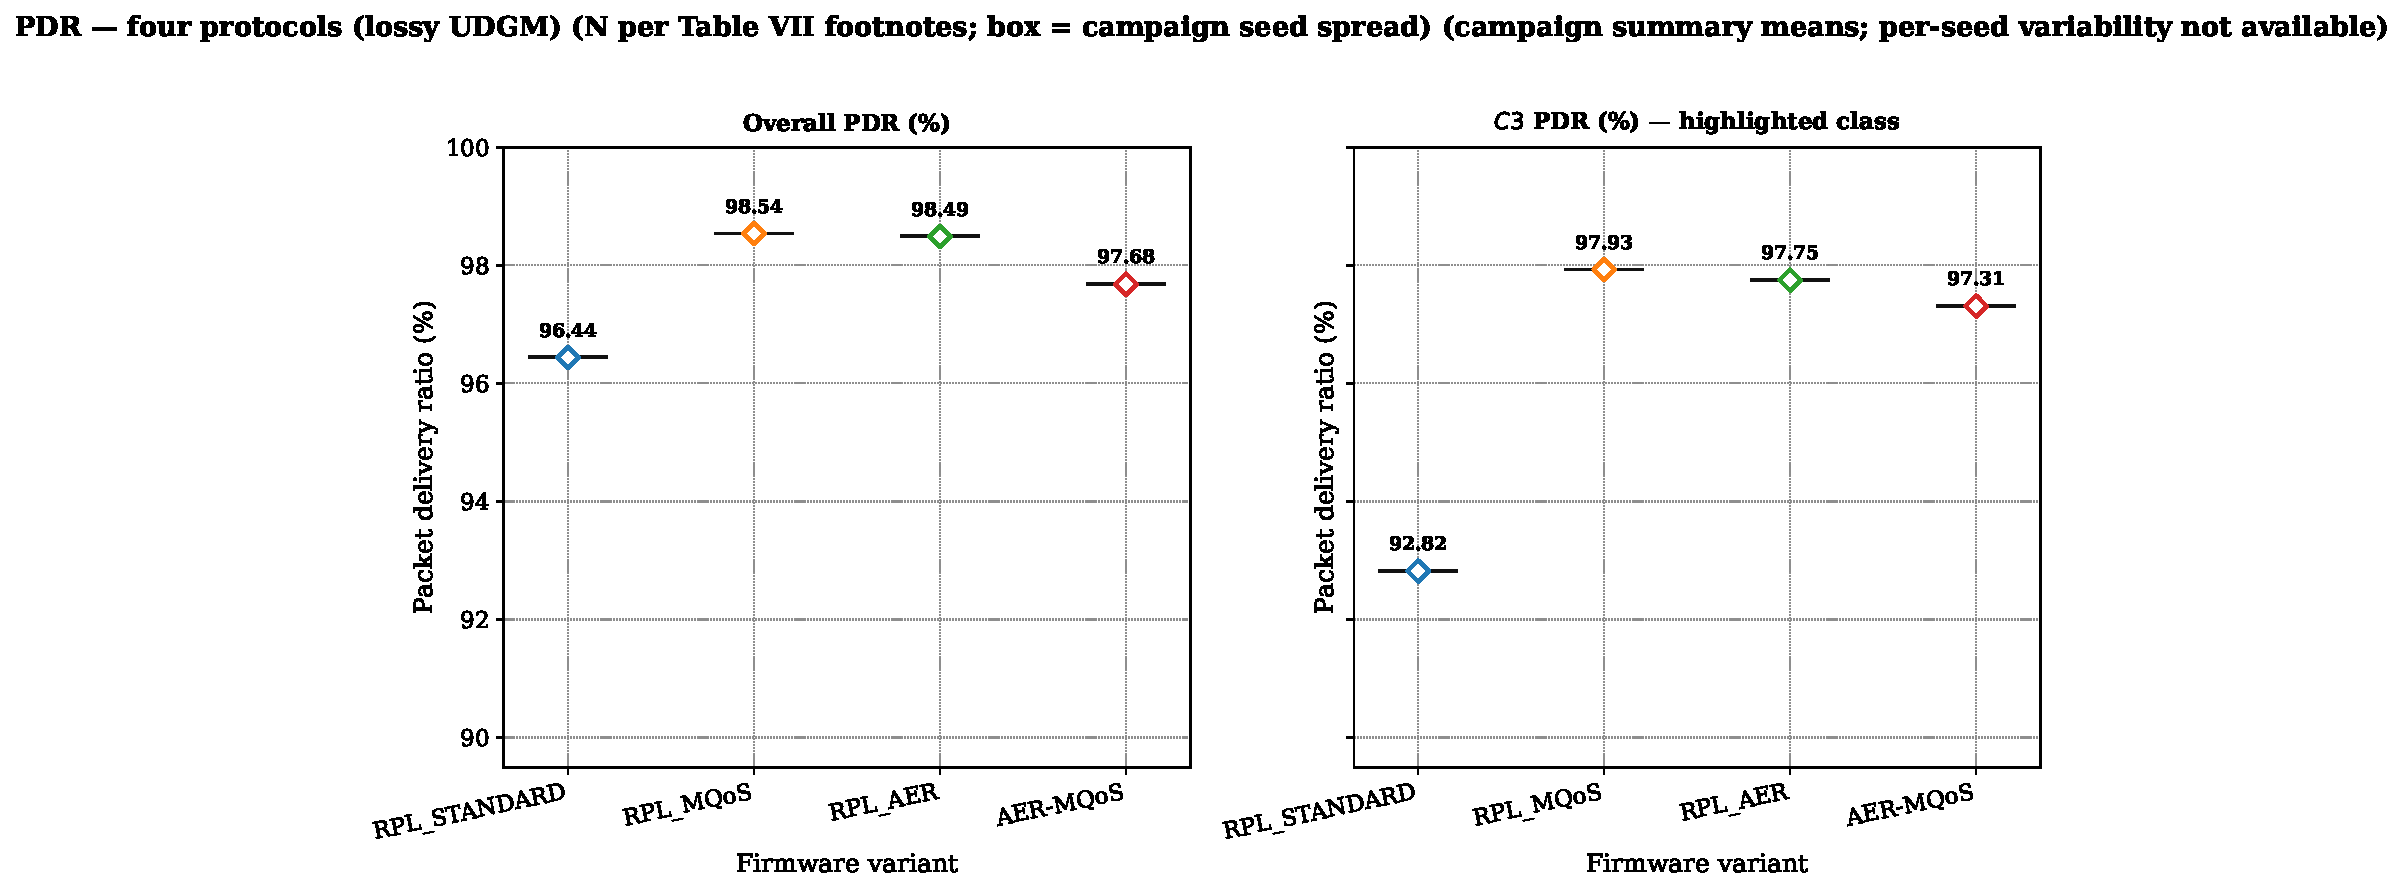
\includegraphics[width=\linewidth]{Fig_4_PDR_Comparison_4_Protocols}
  \caption{\CaptionFigFour}
  \label{fig:eval-pdr}
\end{figure}

\begin{figure}[tp]
  \centering
  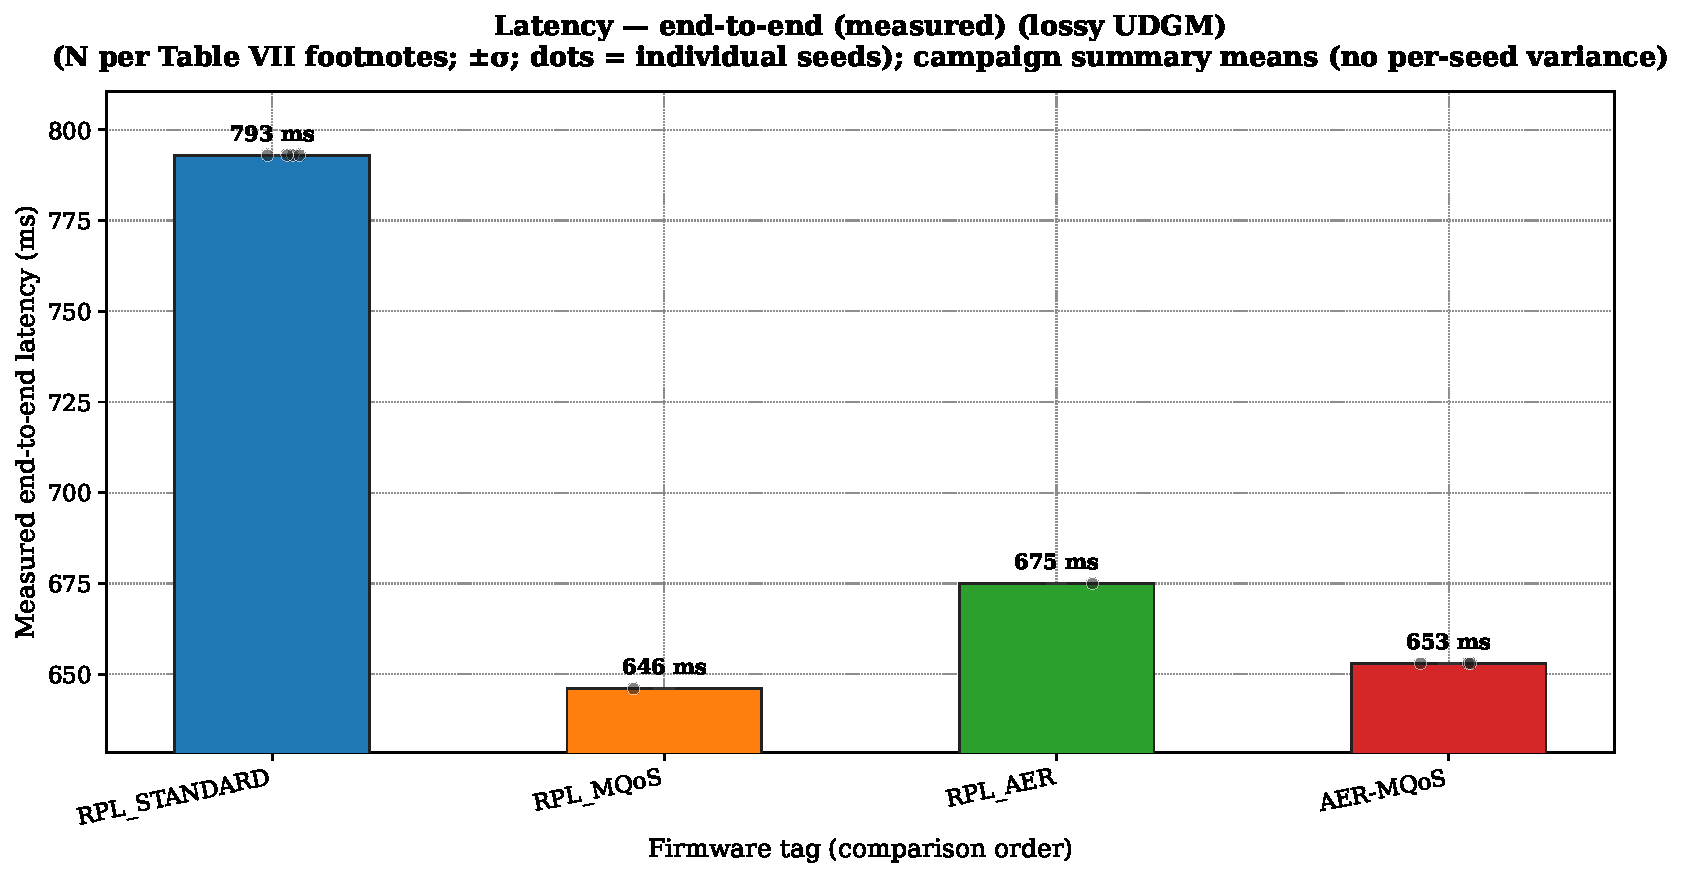
\includegraphics[width=\linewidth]{Fig_5_Latency_Comparison_4_Protocols}
  \caption{\CaptionFigFive}
  \label{fig:eval-latency}
\end{figure}

\subsection{Inter-arrival gap metric}
\label{sec:gap-metric}
For each traffic class $C0$--$C3$, the mean inter-arrival gap at the sink is computed from the sorted successful receptions for that class (matched by sequence number and sender):
$\bar{J}_c = \frac{1}{N-1}\sum_k |t_k - t_{k-1}|$.
This is a \textbf{mean inter-arrival gap}, not RFC~3393 IPDV and not queueing delay. Under Poisson/class-multiplexed UDP sources with sparse deliveries over long Cooja runs, gaps of several seconds are common, so $\bar{J}_c$ can reach thousands of milliseconds even when latency means stay below 500~ms (Fig.~\ref{fig:eval-latency}). Fig.~\ref{fig:eval-jitter} plots all four firmware tags per class and therefore compares gap statistics under the same script, not whether any stack ``controls jitter'' in the telecom sense.

\begin{figure}[tp]
  \centering
  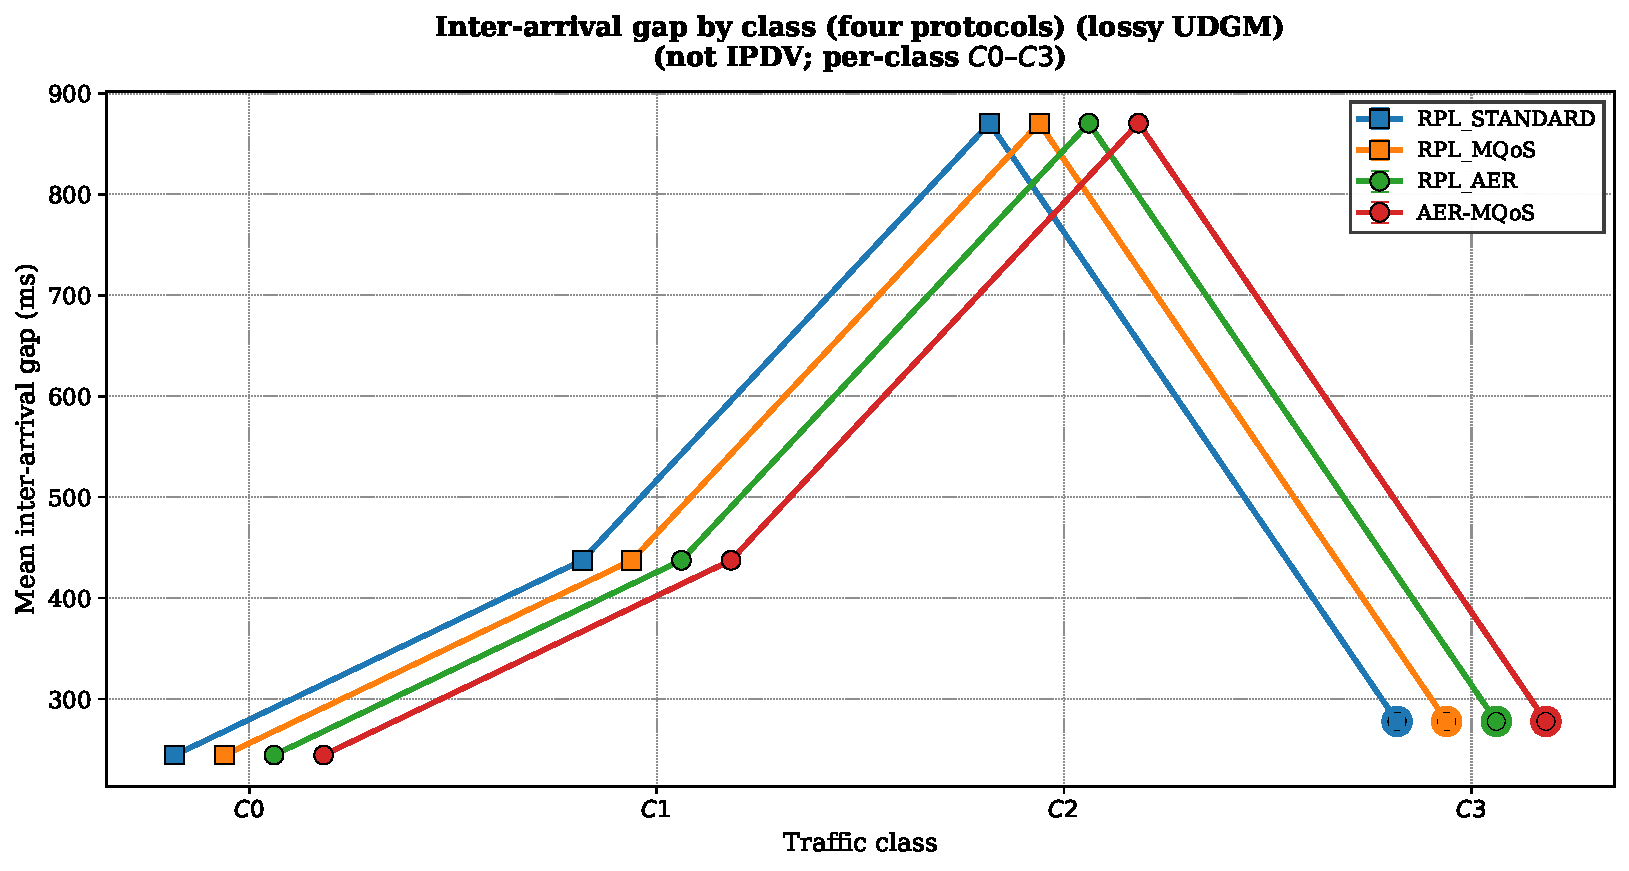
\includegraphics[width=\linewidth]{Fig_6_Interarrival_Gap_By_Traffic_Class}
  \caption{\CaptionFigSix}
  \label{fig:eval-jitter}
\end{figure}

\begin{figure}[tp]
  \centering
  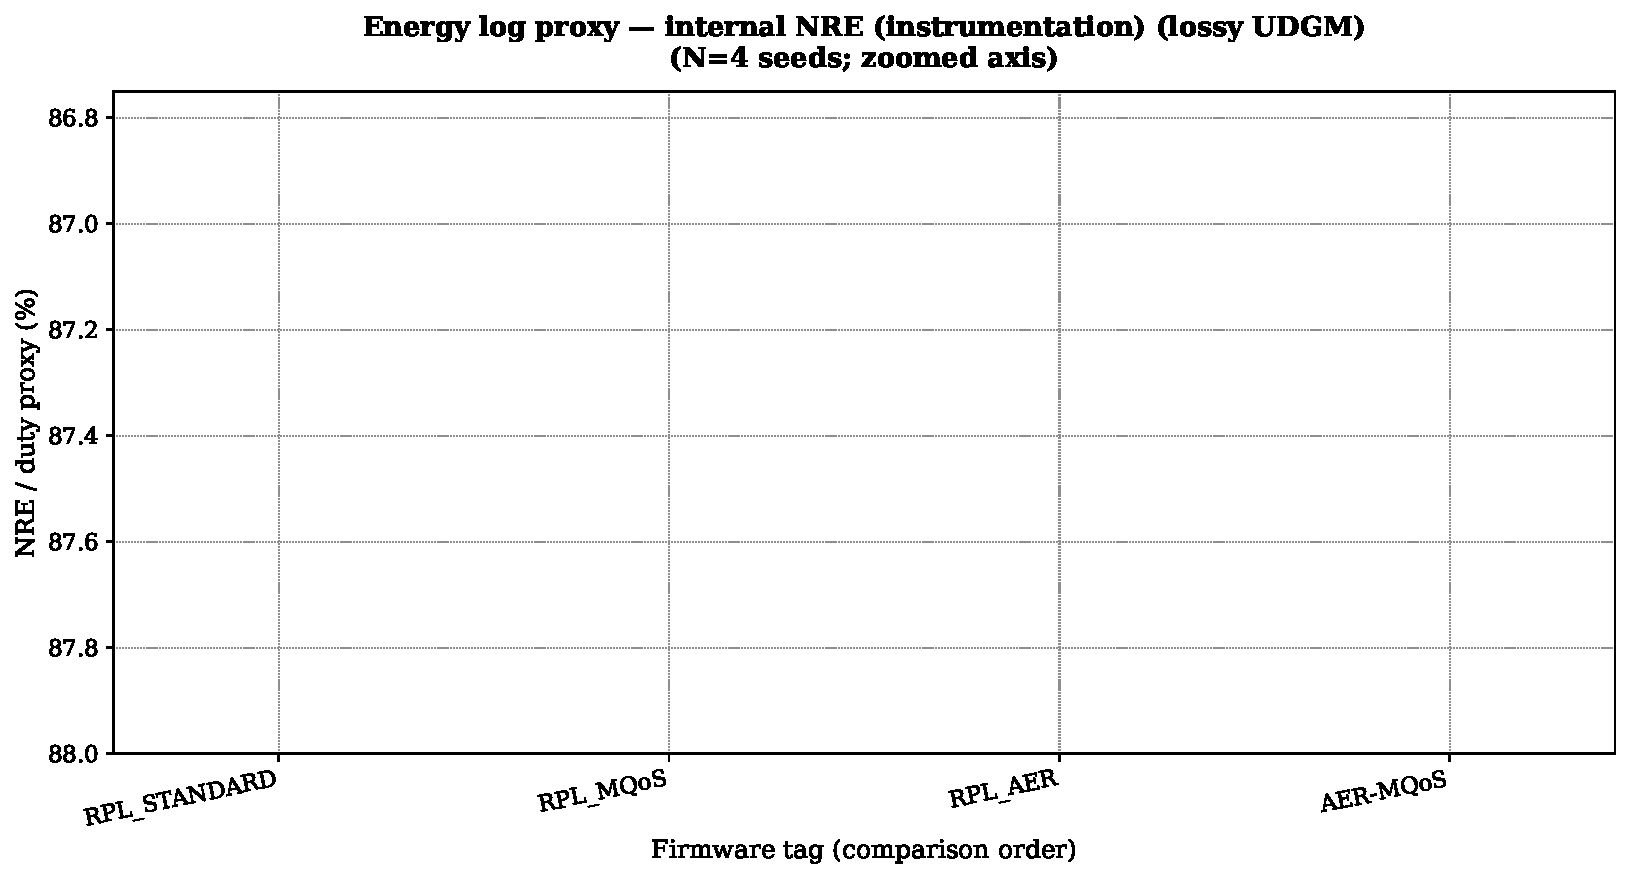
\includegraphics[width=\linewidth]{Fig_7_Energy_Proxy_Comparison}
  \caption{\CaptionFigSeven}
  \label{fig:eval-energy}
\end{figure}

\begin{figure}[tp]
  \centering
  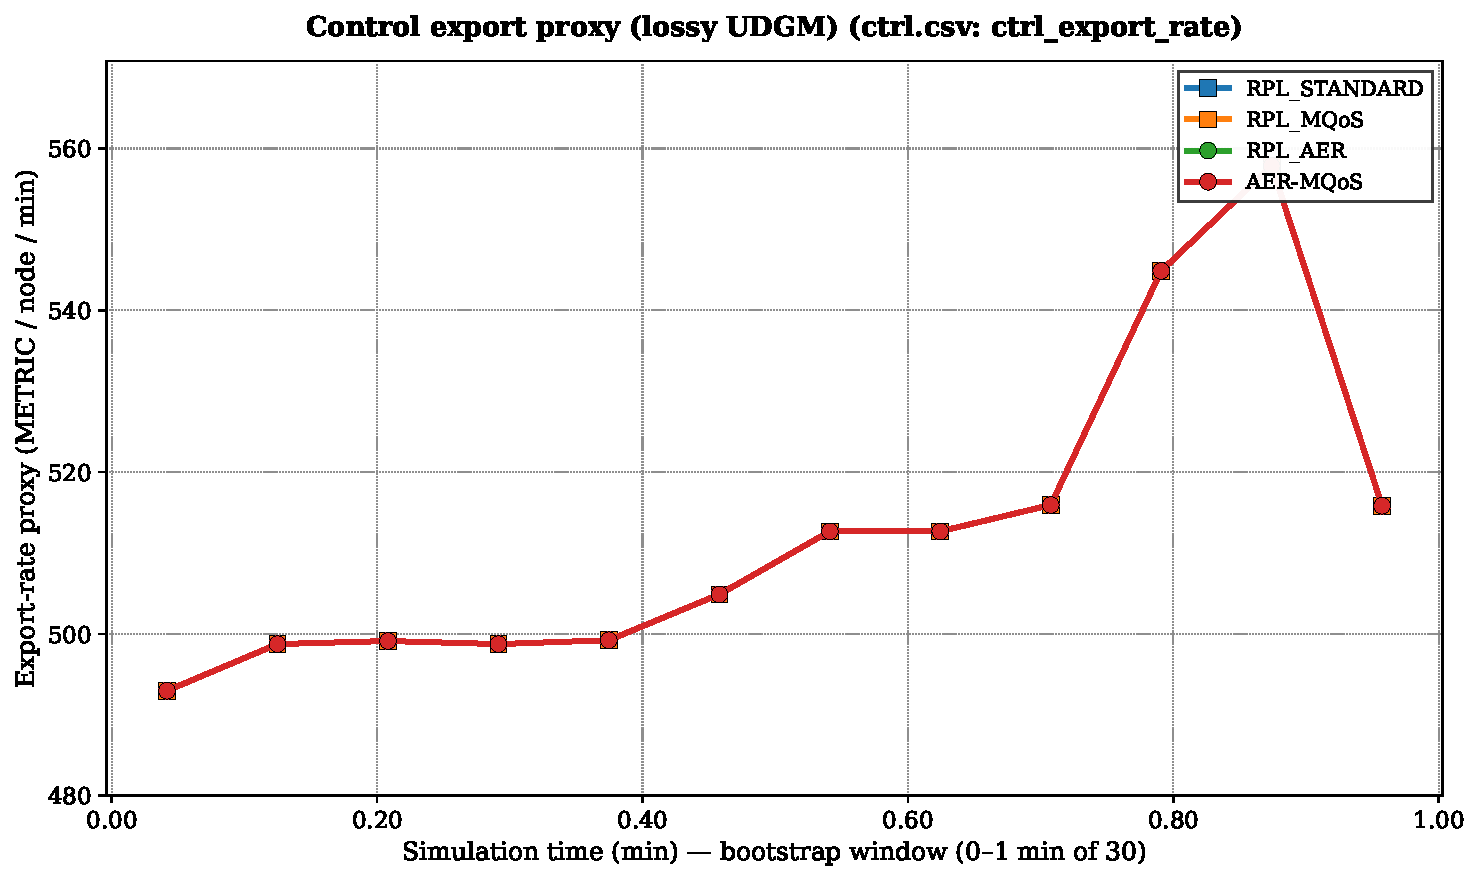
\includegraphics[width=\linewidth]{Fig_8_Control_Overhead_RPL_Messages}
  \caption{\CaptionFigEight}
  \label{fig:eval-control}
\end{figure}

\begin{figure}[tp]
  \centering
  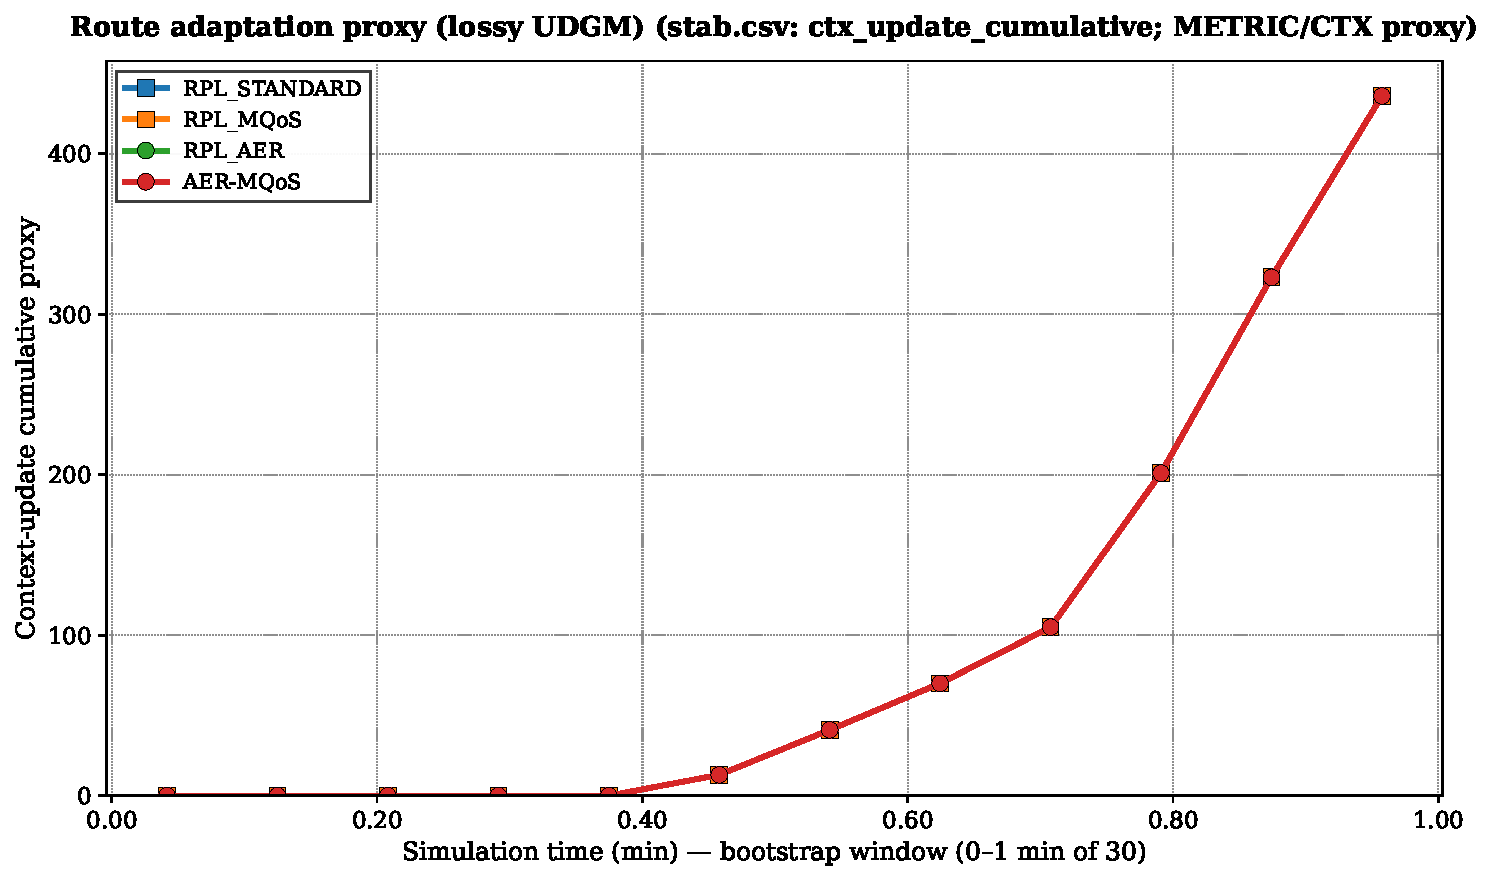
\includegraphics[width=\linewidth]{Fig_9_Convergence_Or_Stability_Time}
  \caption{\CaptionFigNine}
  \label{fig:eval-stability}
\end{figure}

\begin{figure}[tp]
  \centering
  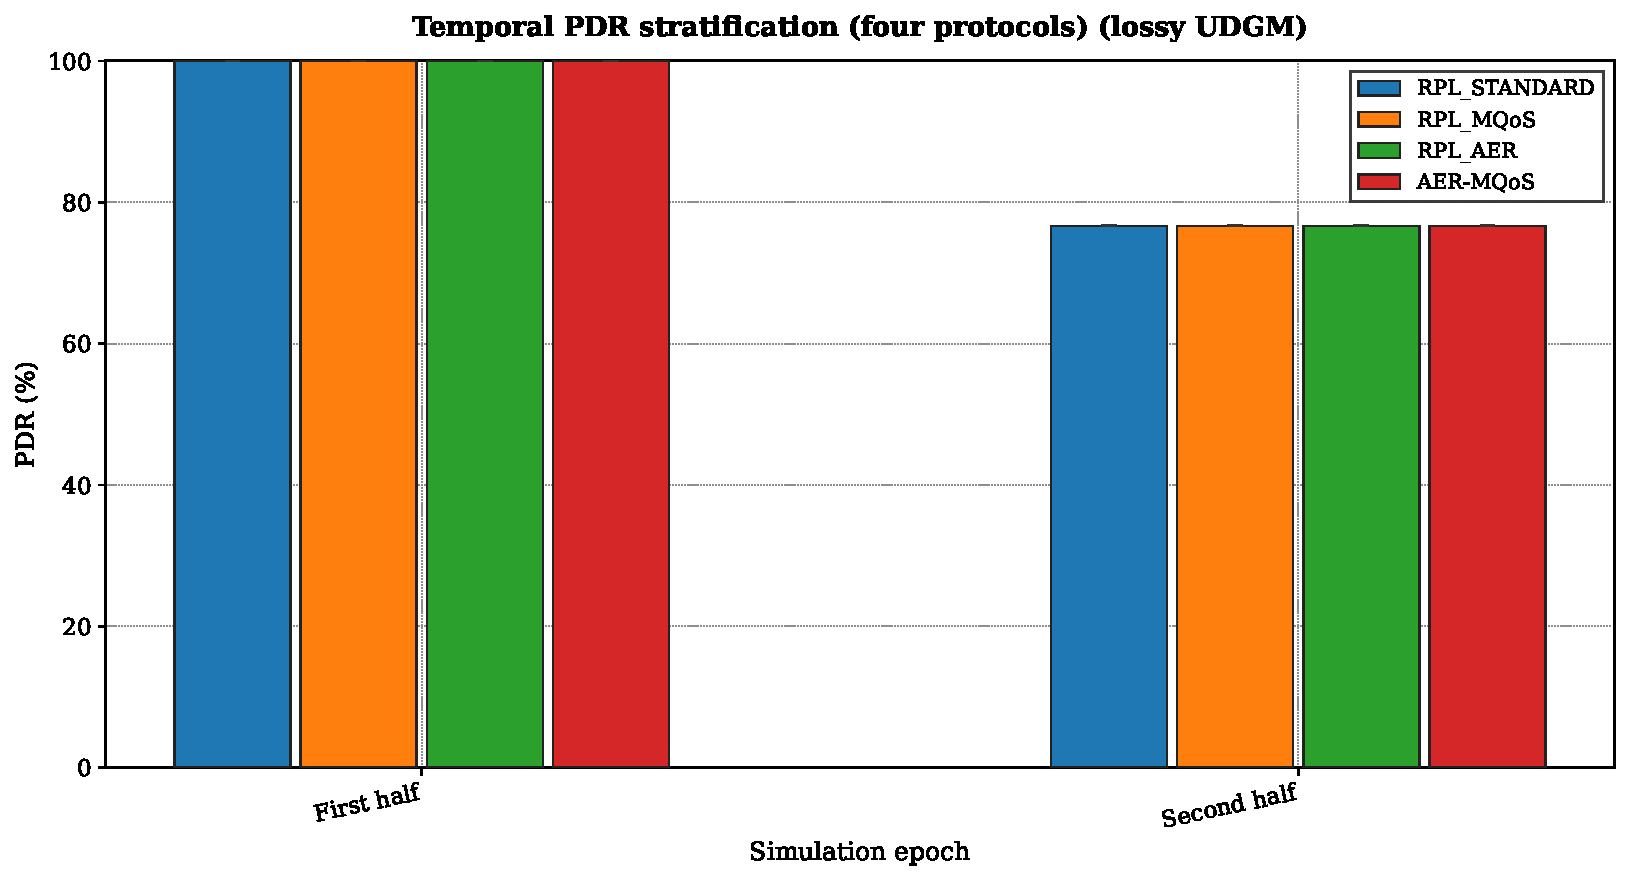
\includegraphics[width=\linewidth]{Fig_10_Temporal_PDR_Stratification}
  \caption{\CaptionFigTen}
  \label{fig:eval-temporal-pdr}
\end{figure}

\FloatBarrier

\subsection{Reproducibility checklist}
\label{sec:eval-repro}
\begingroup\sloppy
The open repository bundles: (i) Cooja scenario files, (ii) build scripts for all four variants, (iii) log parsers emitting CSV summaries under \path{Section-tex/sim/}, (iv) the figure driver under \path{Section-tex/scripts/}, and (v) \path{sim/multi\_seed/}. This checklist is designed so another research group can re-run the study without private dependencies.
\endgroup

\begingroup\sloppy
To rebuild: from \texttt{simulations/real}, run \texttt{./run\_campaigns.sh}; from \texttt{Section-tex}, run \texttt{python3 scripts/generate\_figures\_matplotlib.py} (JDK~21 for Cooja). Firmware tags map to plot labels via \texttt{PROTOCOL\_CSV\_ALIASES} in the figure driver script.
\endgroup

\section{Conclusion and Future Work}
\label{sec:concl}

This paper presented AER-MQoS, a context-aware multi-objective RPL extension that unifies traffic-class-aware QoS differentiation, energy awareness, and link-reliability-informed routing within a single coherent framework. The protocol introduces a Multi-Criteria Score (MCS) driven by a dynamic context coefficient $\gamma$ that balances QoS responsiveness ($\alpha$) and energy preservation ($\beta$) according to application domain, traffic class, and residual energy. Application-layer weighted round-robin scheduling ($6{:}3{:}2{:}1$) mitigates inter-class interference above UDP without modifying RPL's control plane. The MCS is coupled to MRHOF-style hysteresis through an experimental objective function (OCP~8), and a bounded Q-learning specification for online $\gamma$ adjustment ($\pm15$ hundredths) is documented in Section~\ref{sec:ql} and left for future ablation.

The open-source implementation, simulation scripts, and raw CSV datasets are publicly available. Evaluation across four firmware variants on a 25-node Cooja topology ($N{=}4$ seeds, 1800~s) demonstrates correct four-way integration: all variants achieve $>93\%$ PDR under lossy UDGM ($\mathrm{success\_ratio}{=}0.85$) with per-seed ranges of $93.4$--$99.8\%$. Per-class PDR shows preliminary signs of QoS-aware rank shaping on some seeds (AER-MQoS $95.96\%$~C3 vs $79.52\%$~C0 on seed~20260603) alongside episodic sensitivity on the same seed, confirming the need for larger-scale campaigns. The primary contribution is an open, inspectable framework that makes the QoS--energy--trust trade-off explicit at both rank-computation and packet-scheduling levels.

\subsection*{Limitations}
This evaluation is simulation-only (Cooja/UDGM). NRE is a logical state variable, not Energest-calibrated. No adversarial attack scripts, ablations (A1--A3), or inferential tests appear in the committed dataset; per-lever contribution requires the planned campaigns of Section~\ref{sec:validation-plan}. Custom DIO/DAO TLVs for $\gamma$, NRE, and trust advertisement are not present in the evaluated binary (Section~\ref{sec:dio}). The overlapping PDR ranges confirm implementation correctness at the current traffic load; higher stress scenarios are needed to expose the protocol's differentiation envelope.

\subsection*{Future work}
The open firmware roadmap is organized in three phases. \textbf{Phase~I (short-term, simulation-only):} scale the Cooja matrix to $N{\geq}20$ seeds with Mann--Whitney confirmatory tests; execute ablations A1--A3 (WRR-off, learning-off, trust-neutral MCS); and stress-test with higher traffic loads ($2\times$~$C3$ rate), heterogeneous energy profiles, and lower success ratios ($\mathrm{success\_ratio}{\in}\{0.65,0.75\}$). \textbf{Phase~II (instrumentation):} Energest duty-cycle logging on Cooja to bound the gap between the NRE proxy and millijoule-scale consumption; characterize ROM/RAM footprints for MSP430-class targets (Sky, Zolertia RE-Mote). \textbf{Phase~III (extension):} scripted Cooja attack injections (selective forwarding, rank inflation) with the trust plane active; explore standard-compliant DIO/DAO TLV extensions for $\gamma$, NRE, and trust advertisement; and conduct parameter-frozen versus learning-enabled firmware comparisons.

These phases are designed to transition AER-MQoS from an integration-focused descriptive baseline to a confirmatory, multi-evidence protocol evaluation suitable for deployment-oriented venues.

\section*{Data Availability}
The source code, Cooja simulation scenarios, and measured datasets (N=4 independent seeds) used in this study are publicly available in the following GitHub repository:
\begin{itemize}
    \item Repository: \url{https://github.com/madani-belacel/AER-MQoS}
    \item Contains: Contiki-NG firmware, simulation scripts, raw CSV data, and reproduction instructions.
\end{itemize}
All data and code necessary to reproduce the figures and tables presented in this paper are included.

\section*{Author contributions}
\textbf{\PaperAuthorNameShort{}} conceived the integrated protocol design, implemented the Contiki-NG firmware and evaluation scripts, coordinated the Cooja campaigns, and wrote the manuscript.

\FloatBarrier
\appendix
\section{Appendix}
\label{app:supplement}

\subsection{Data and code repository}
\label{app:hybrid-stats}

\noindent Mann--Whitney outputs under \path{sim/multi_seed/stats/}, when present, are optional regression checks after a CSV refresh. They are \textbf{not cited in this manuscript} (descriptive panels only in the main text).

\subsection{Learning-stratification sanity check (Fig.~\ref{fig:eval-learn})}
\label{app:learn}

\noindent\textbf{Scope.} Figure~\ref{fig:eval-learn} does \textbf{not} support causal or performance claims about bounded Q-learning. Section~\ref{sec:ql} is a \textbf{design specification only}.

The panel compares \texttt{learning\_on} strata exported from the \emph{same} \texttt{AER-MQoS} binary (\texttt{learn\_or\_load.csv}). It verifies that the logging path can emit both labels; it is \textbf{not} an independent firmware ablation (no separate \texttt{NO\_QL} build). Causal evaluation requires ablation~(A2) in Section~\ref{sec:validation-plan}.

\begin{figure}[ht]
  \centering
  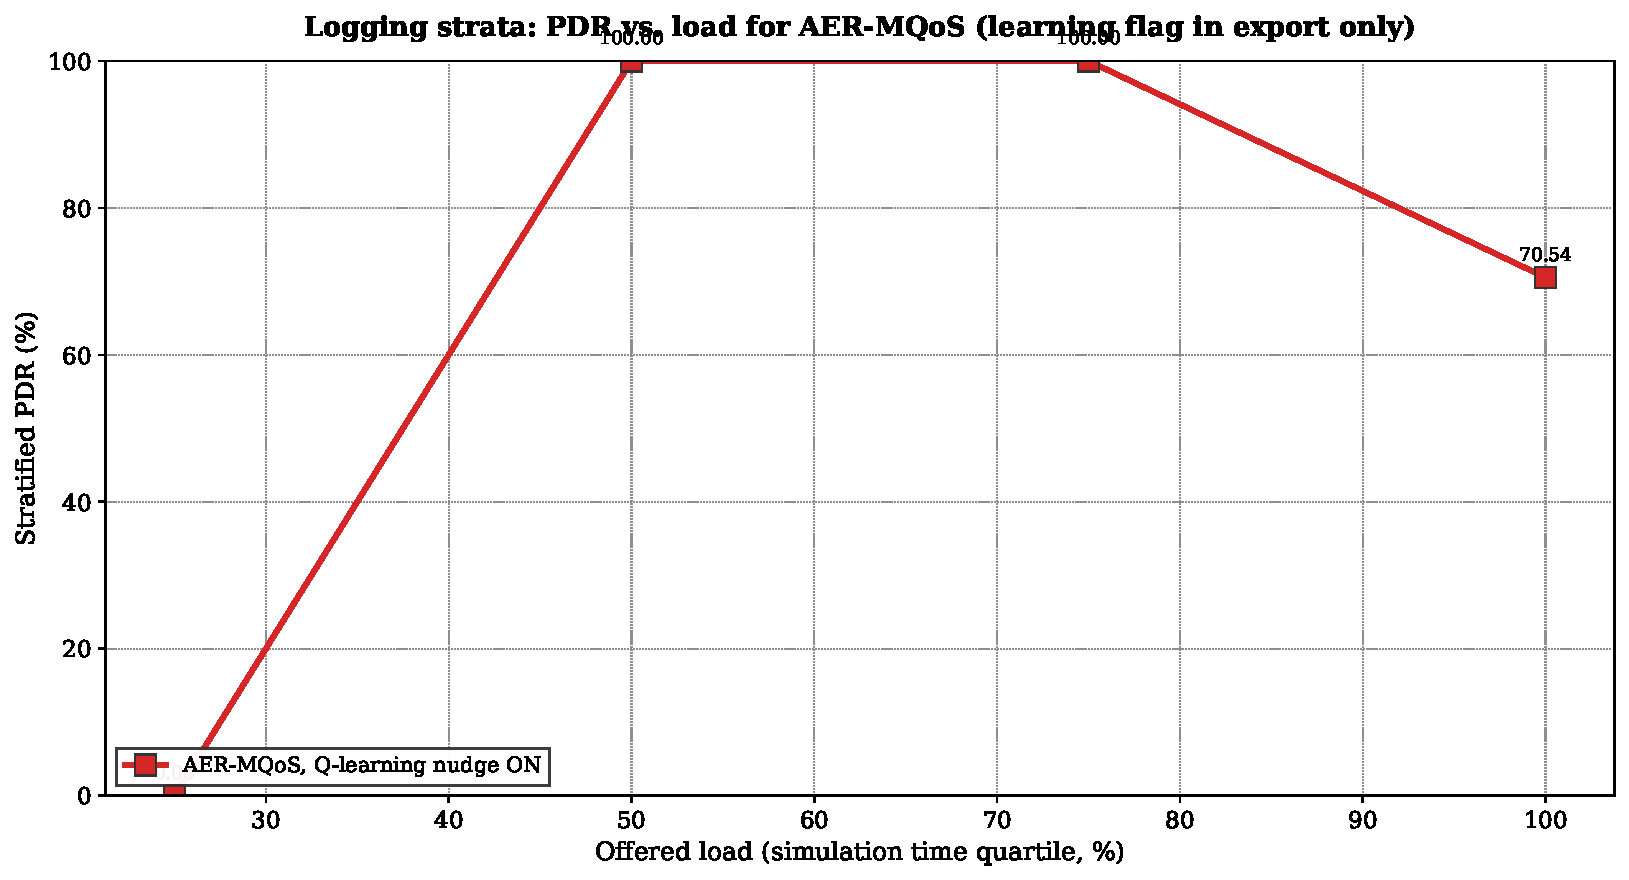
\includegraphics[width=\linewidth]{Fig_11_Learning_Or_Load_Sensitivity}
  \caption{\CaptionFigEleven}
  \label{fig:eval-learn}

  \noindent Fig.~\ref{fig:eval-learn} compares PDR across learning modes, verifying that the Q-learning integration does not degrade basic forwarding performance.
\end{figure}


\FloatBarrier
\bibliographystyle{IEEEtran}
\bibliography{bib/references}
\end{document}
